
\documentclass[aspectratio=169]{beamer}
\usetheme{metropolis}           % Use metropolis theme
\usepackage[utf8]{inputenc}
\usepackage{graphicx}
\usepackage{eso-pic}
\usepackage{graphics}
\usepackage{tikz}
\usepackage[export]{adjustbox}
\usepackage{multicol}
\usepackage{listings}
\usepackage{helvet}
\usepackage{booktabs}
\usepackage{threeparttable}
\usepackage{upquote}

\title{Data Visualization}
\date{\today}
\author{Author of Session here!} % Name of author(s) of session here
\institute{Development Impact Evaluation (DIME) \newline The World Bank }
\setbeamercolor{background canvas}{bg=white}	% Sets background color

% The below command places the World Bank logo and DIME logo to the right corner
\titlegraphic{%
	\begin{picture}(0,0)
	\put(330,-180){\makebox(0,0)[rt]{
\includegraphics[width=3cm]{img/WB_logo}}}
	\end{picture}%
	\begin{picture}(0,0)
	\put(390,-180){\makebox(0,0)[rt]{
\includegraphics[width=1.5cm]{img/i2i}}}
	\end{picture}%
}

%%% Section page with picture of Light bulb
\makeatletter
\defbeamertemplate*{section page}{mytheme}[1][]{
	\centering
	\begin{minipage}{22em}
		\raggedright
		\usebeamercolor[fg]{section title}
		\usebeamerfont{section title}
		\par
		\ifx\insertsubsectionhead\@empty\else%
		\usebeamercolor[fg]{subsection title}%
		\usebeamerfont{subsection title}%
		\fi
		\ifstrempty{#1}{}{%
			\includegraphics[width=100mm, height=60mm]{#1}%
		}
		\insertsectionhead\\[-1ex]
		\insertsubsectionhead
		\usebeamertemplate*{progress bar in section page}
		
	\end{minipage}
	\par
	\vspace{\baselineskip}
}
\makeatother

%%% Define a command to include picture in section, 
%%% make section, and revert to old template
\newcommand{\sectionpic}[2]{
	\setbeamertemplate{section page}[mytheme][#2]
	\section{#1}
	\setbeamertemplate{section page}[mytheme]
}

%%% The command below allows for the text that contains Stata code
\lstset{ %
	backgroundcolor=\color{white},
	basicstyle=\tiny,
	breakatwhitespace=false,
	breaklines=true,
	captionpos=b,
	commentstyle=\color{green},
	escapeinside={\%*}{*)},
	extendedchars=true,
	frame=single,
	numbers=left,
	numbersep=5pt,
	numberstyle=\tiny\color{gray},
	rulecolor=\color{black},
	showspaces=false,
	showstringspaces=false,
	showtabs=false,
	stringstyle=\color{mauve},
	tabsize=2,
	title=\lstname,
	morekeywords={not,\},\{,preconditions,effects },
	deletekeywords={time}
}

%% The below command creates the ligh bulb logos in the top right corner of the 
\begin{document}
	
{
	\usebackgroundtemplate{
\includegraphics[height=55mm, right]{img/top_right_corner.pdf}}
	\maketitle
}


\begin{frame}{Tables give all the details}
	\begin{multicols}{2}	
	
	\begin{itemize}[<default overlay specification>]
		\item<1> What’s happening in this regression table? What’s important?
	\end{itemize}
	
	\begin{figure}
		\centering
		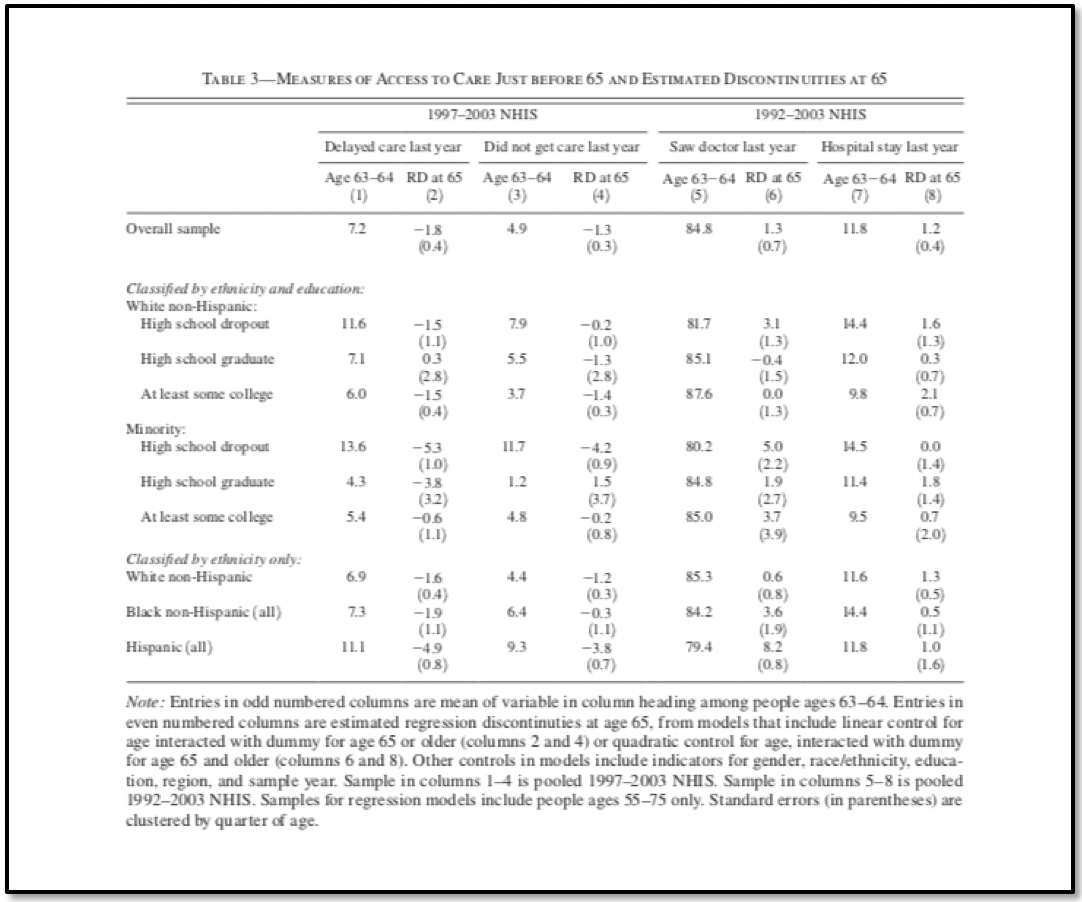
\includegraphics[width=60mm]{img/Table}
	\end{figure}
	
\end{multicols}
\end{frame}

\begin{frame}{But figures tell the story}
	\begin{multicols}{2}	
		
		\begin{itemize}[<default overlay specification>]
			\item<1> This is the data that generates those estimates.
			\item<1> You can see exactly what is happening very quickly!
		\end{itemize}
	
	Even more importantly: You don't have to look for it. The eye is drawn to the story!
		
		\begin{figure}
			\centering
			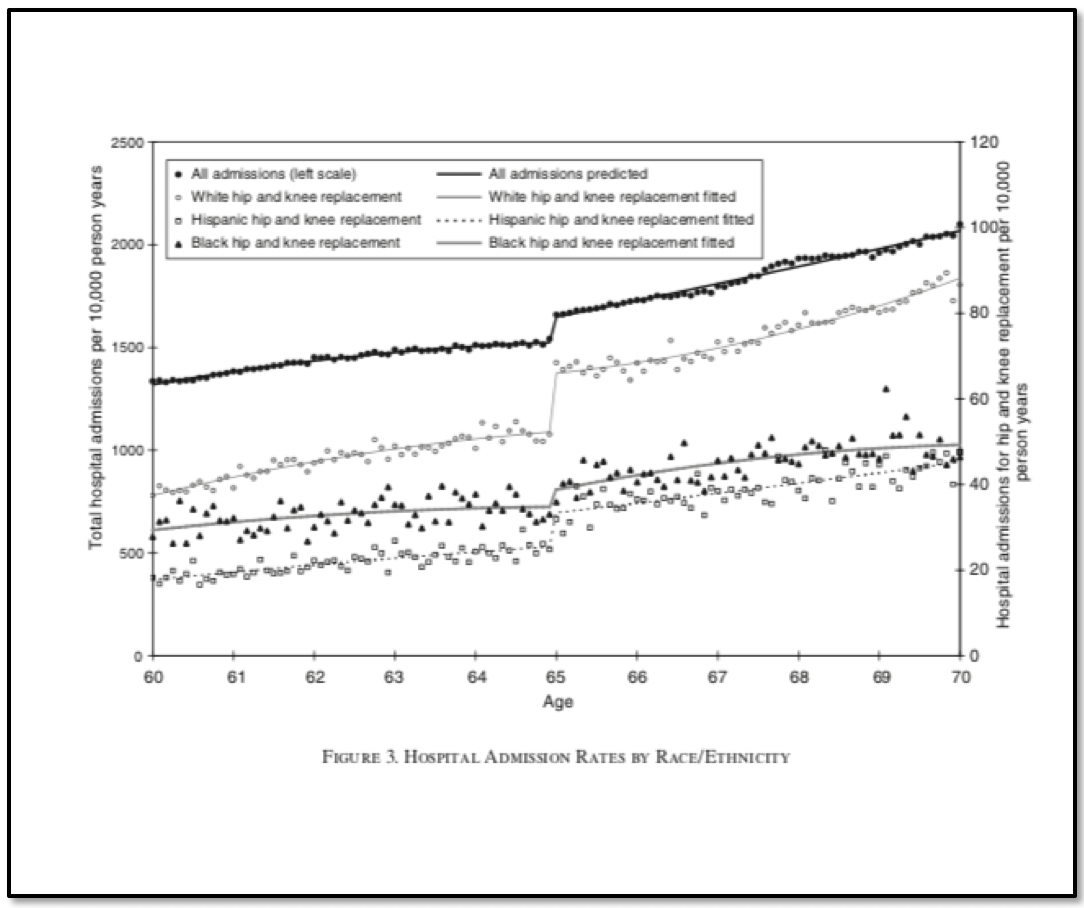
\includegraphics[width=60mm]{img/Table2}
		\end{figure}
		
	\end{multicols}
\end{frame}


\begin{frame}{Examples: Examining distributions}
	
	\begin{figure}
		\centering
		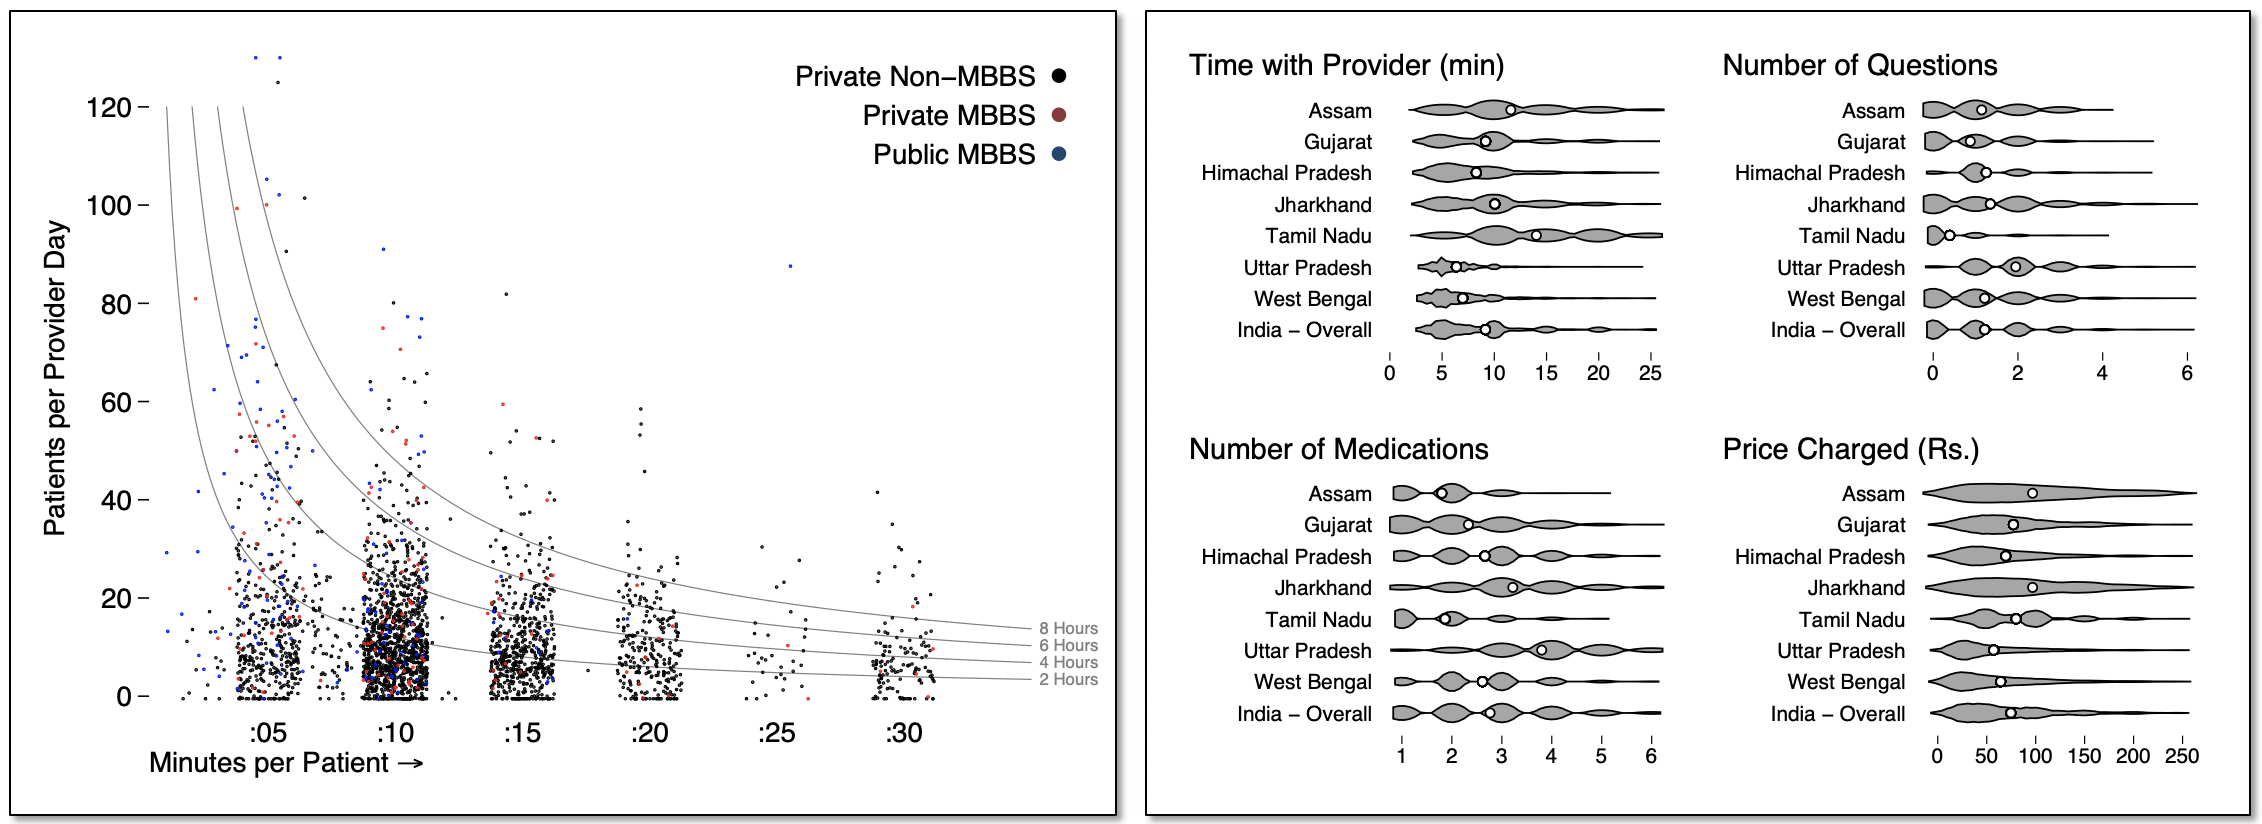
\includegraphics[width=\linewidth]{img/Distribution}
	\end{figure}
	
\end{frame}

\begin{frame}{Examples: Comparing means}
	
	\begin{figure}
		\centering
		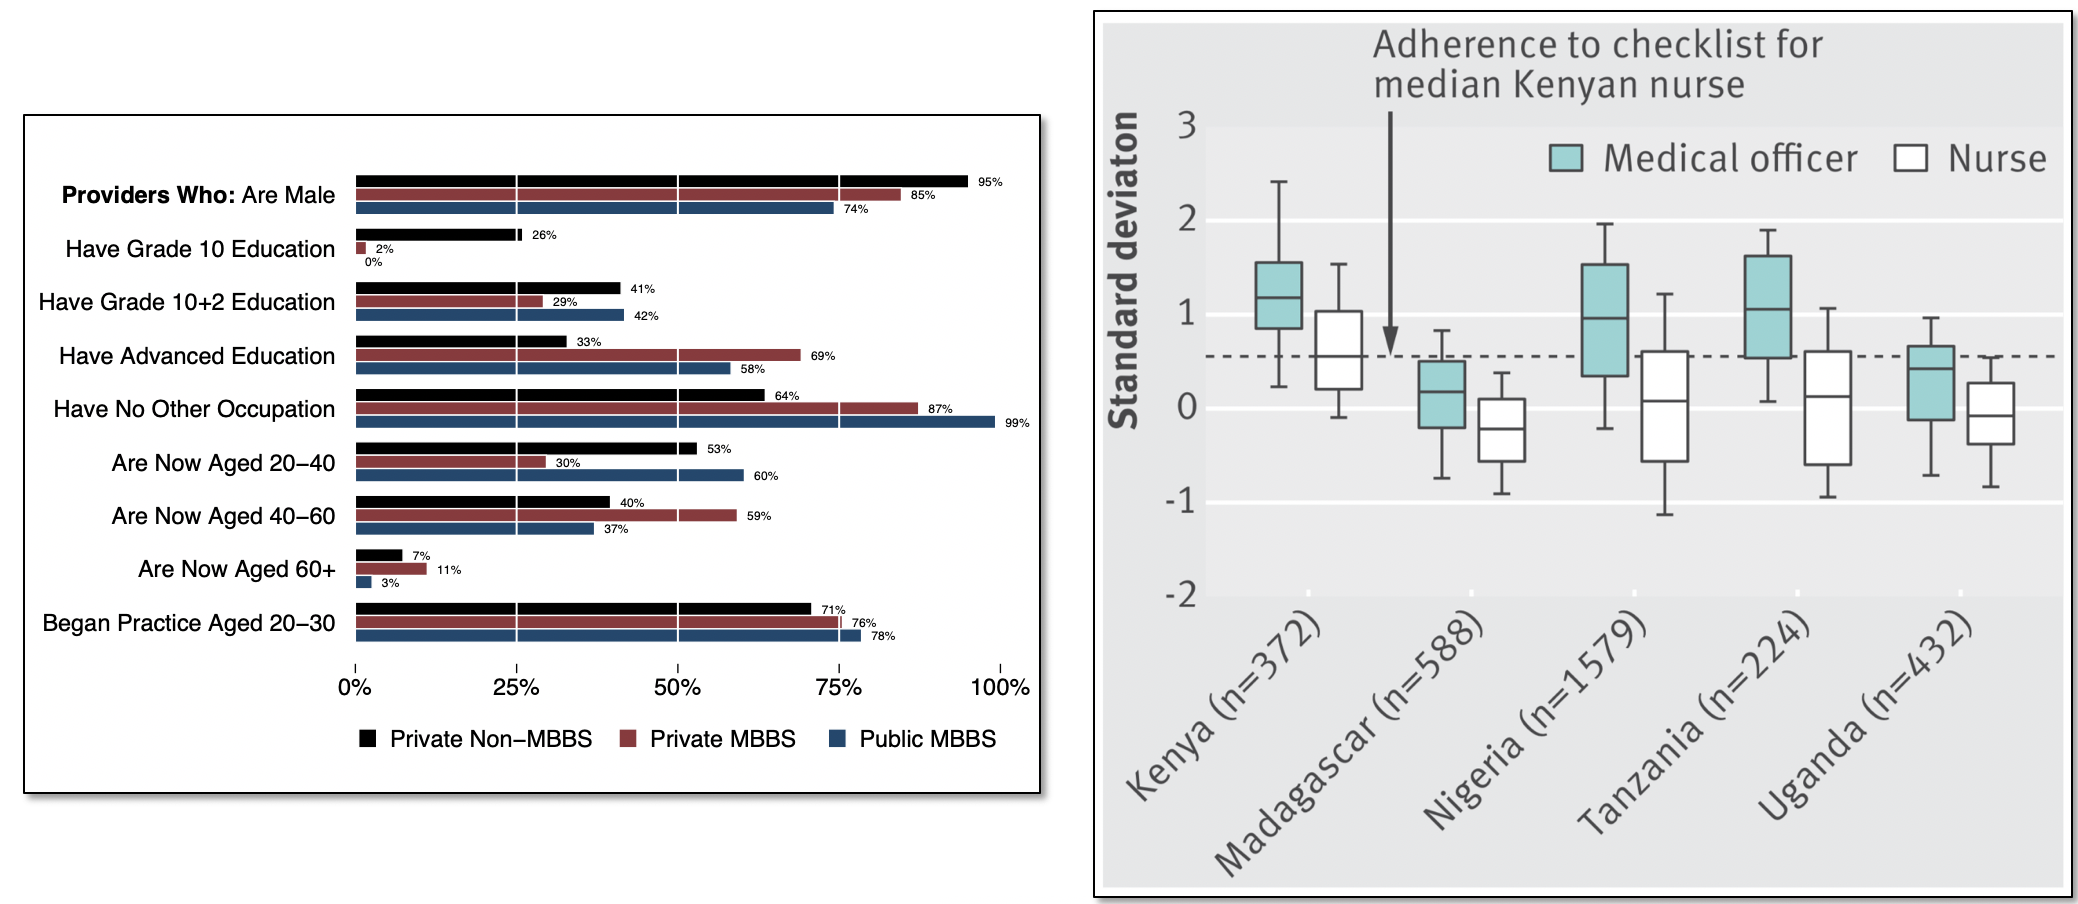
\includegraphics[width=\linewidth]{img/Distribution2}
	\end{figure}
	
\end{frame}


\begin{frame}{Some examples: Comparing correlations}
	
	\begin{figure}
		\centering
		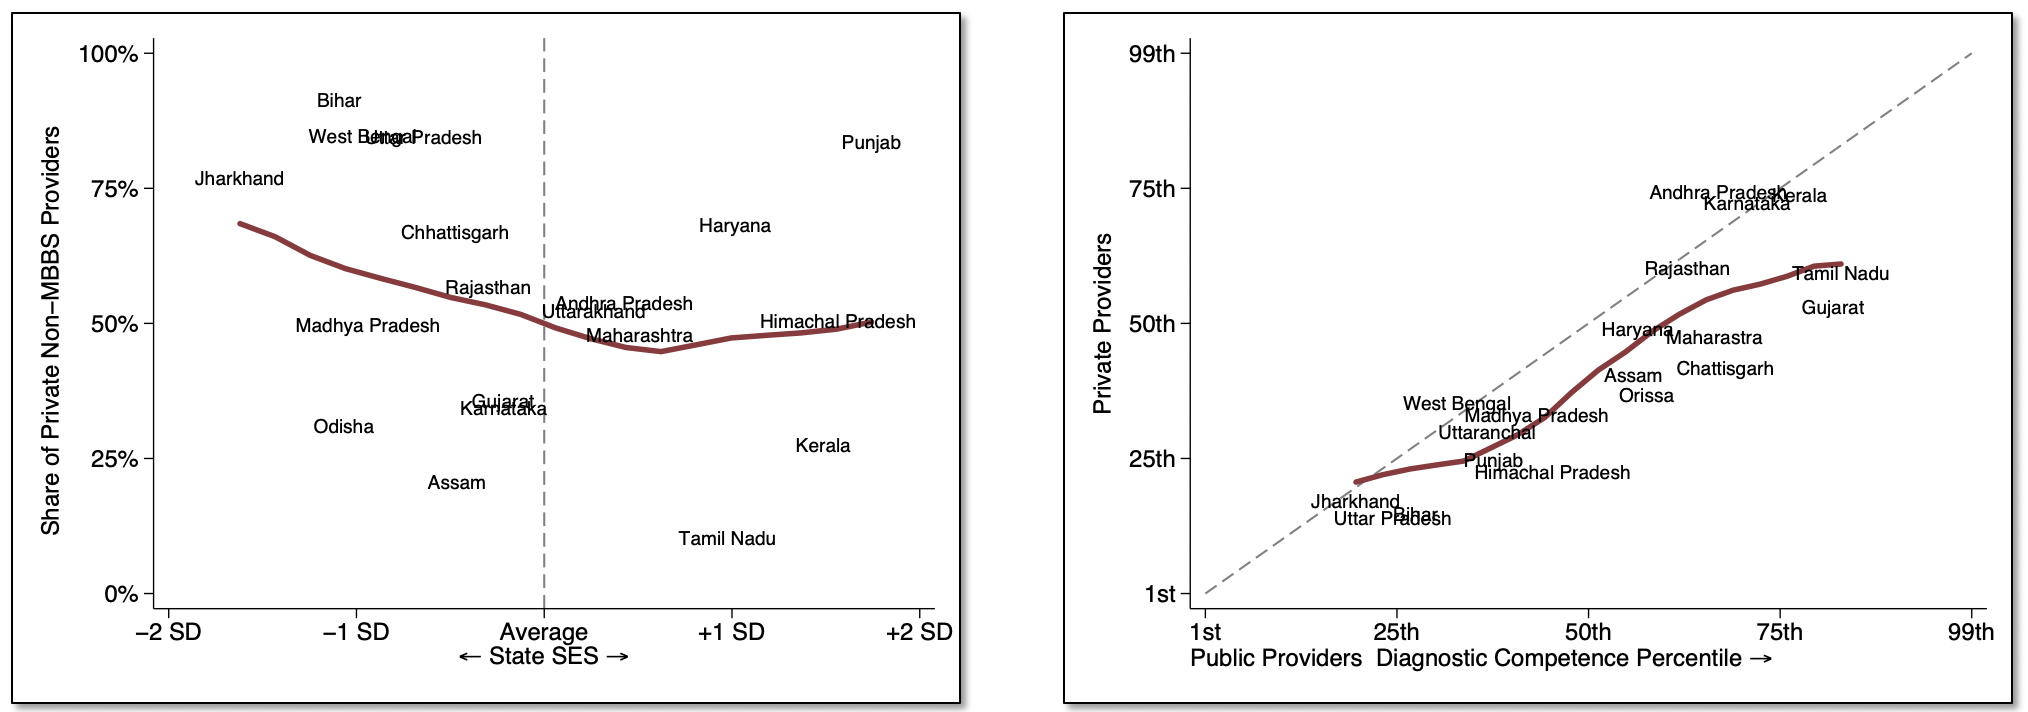
\includegraphics[width=\linewidth]{img/Correlation}
	\end{figure}
	
\end{frame}


\begin{frame}{Some examples: Searching for patterns}
	
	\begin{figure}
		\centering
		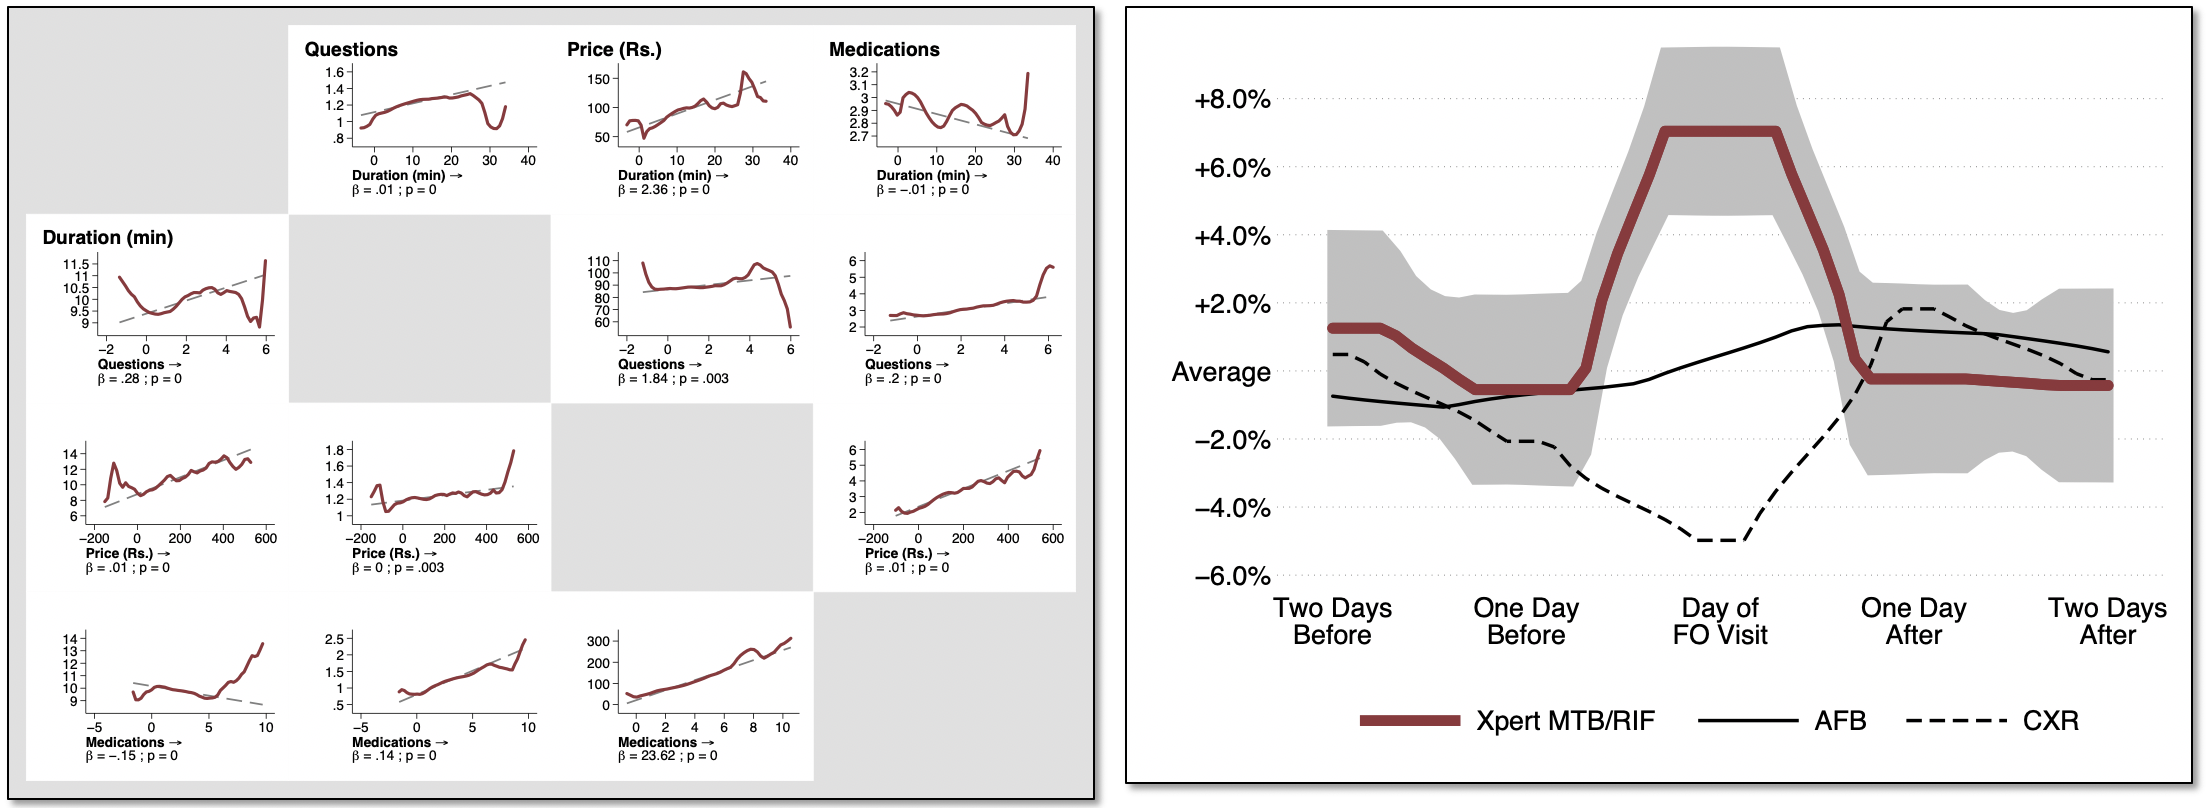
\includegraphics[width=\linewidth]{img/Correlation2}
	\end{figure}
	
\end{frame}


\begin{frame}{Some examples: Telling a story about treatment takeup}
	
	\begin{figure}
		\centering
		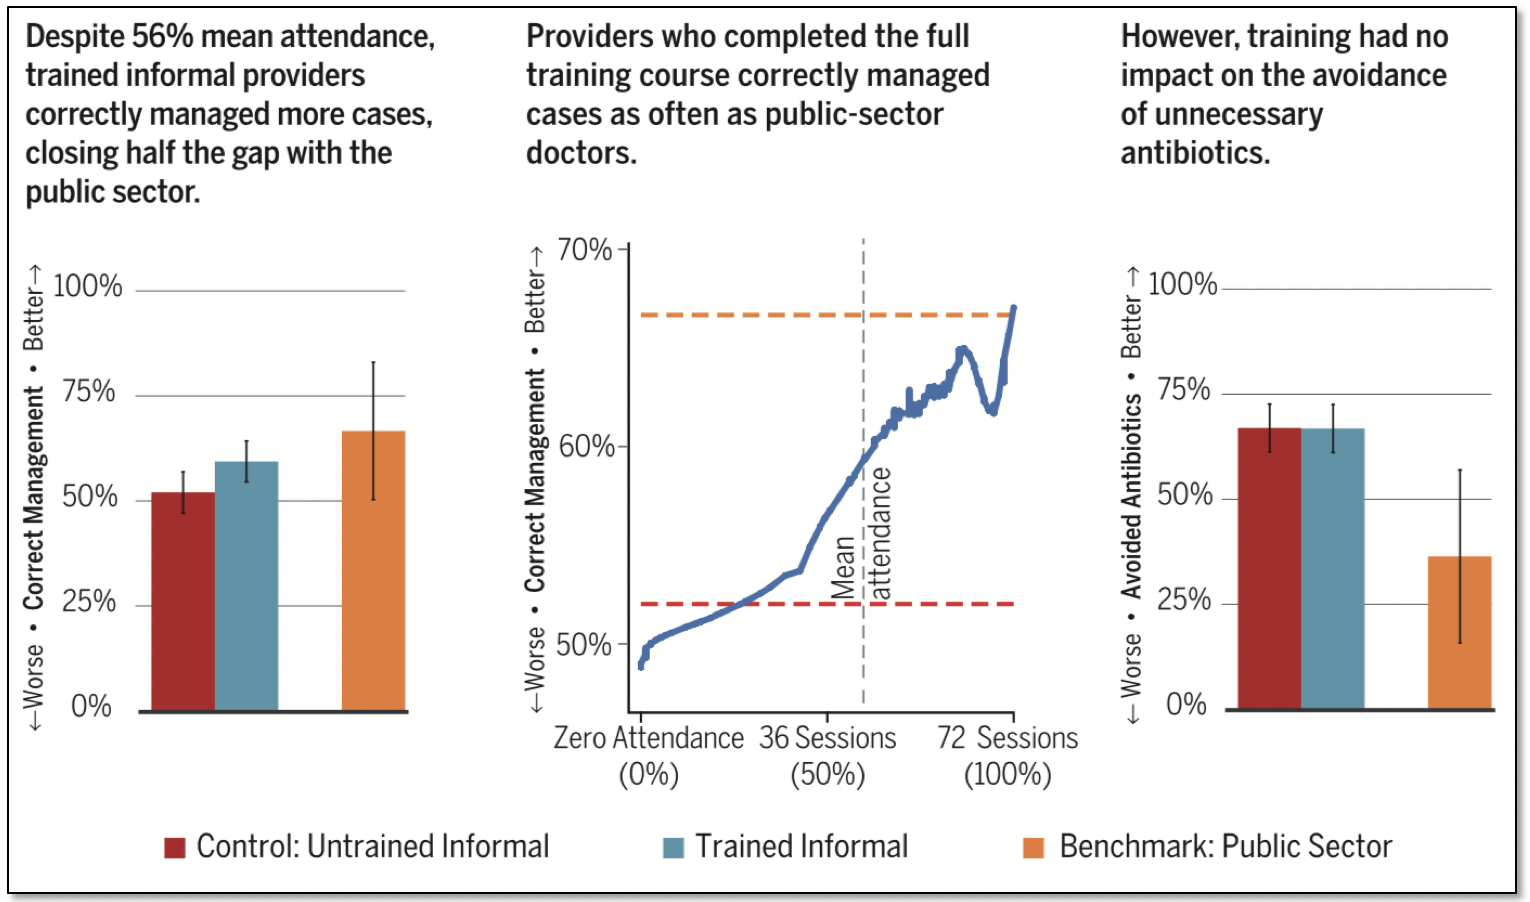
\includegraphics[width=\linewidth]{img/Correlation3}
	\end{figure}
	
\end{frame}


\begin{frame}{Why do these charts look so good?}
		
		\begin{itemize}[<default overlay specification>]
			\item<1> They tell a story.
			\item<1> They use consistent visual (design) language.
			\item<1> They draw the eye to what is important.
		\end{itemize}
		
\end{frame}


\begin{frame}{Stata default graphs are not very attractive}
	
	\begin{figure}
		\centering
		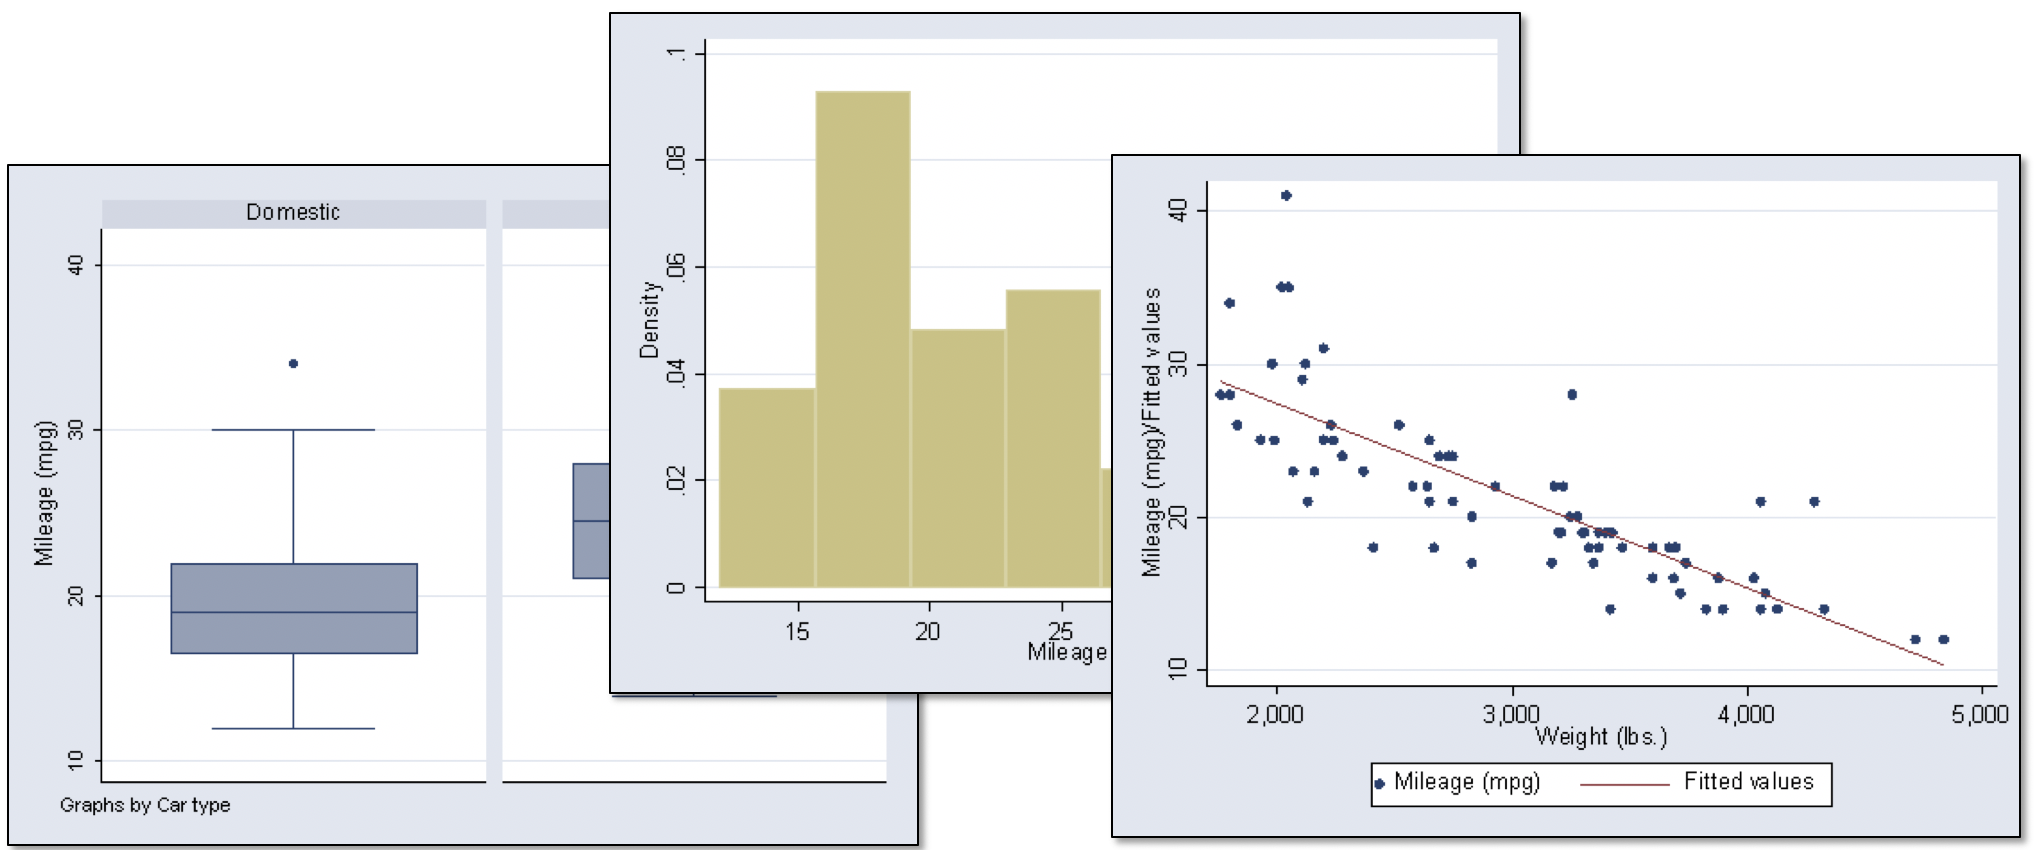
\includegraphics[width=\linewidth]{img/Graph}
	\end{figure}
	
\end{frame}


\begin{frame}{Stata has three core built-in graph functions}
	\begin{multicols}{2}	
			
			\begin{itemize}[<default overlay specification>]
			\item<1> \texttt{graph graphtype}
				\newline - Graph which plot one or more variables on one axis.
			\item<1>  \texttt{twoway graphtype}
				\newline - Graph which two plot variables together on an x,y axis.
			\item<1>  \texttt{histogram, kdensity, lowess}
				\newline - Essential distributional commands.
		\end{itemize}
		
		\begin{figure}
			\centering
			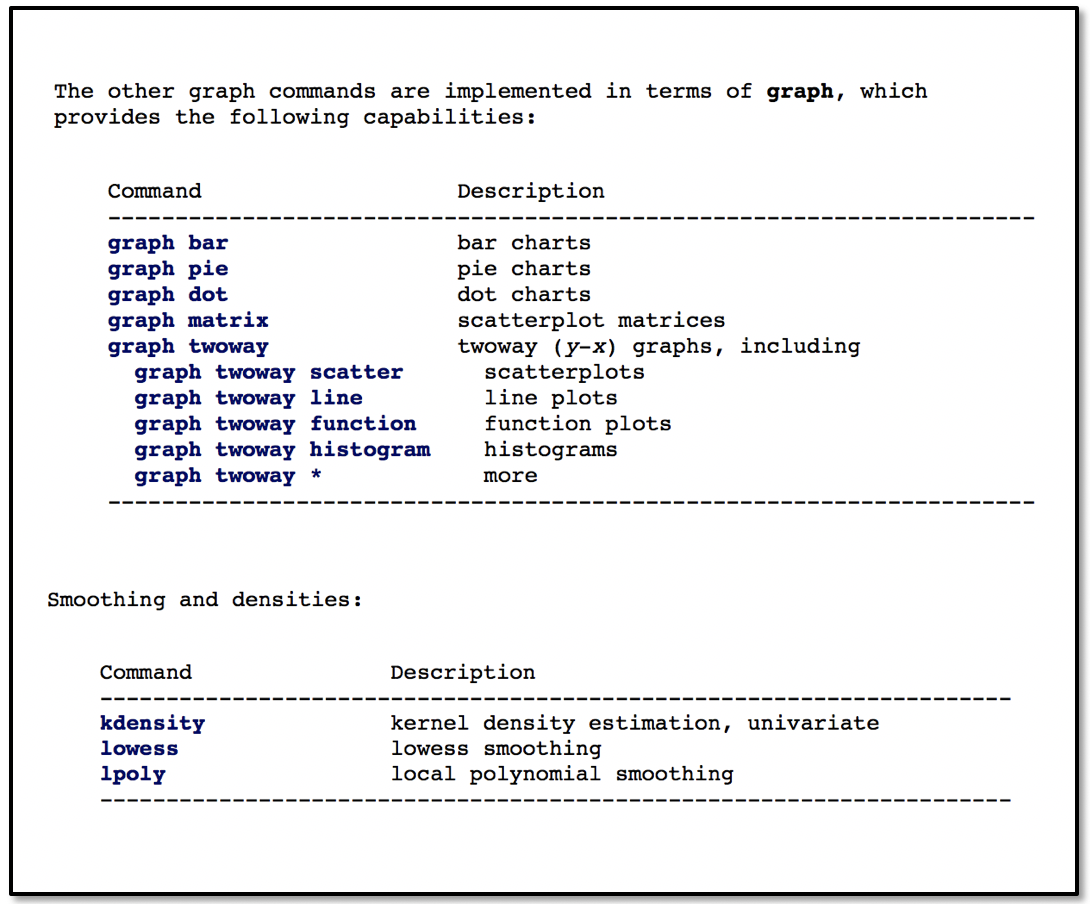
\includegraphics[width=70mm]{img/Function}
		\end{figure}
		
	\end{multicols}
\end{frame}


\begin{frame}{Oneway  \texttt{graph} plots can be very informative}
	
	\begin{figure}
		\centering
		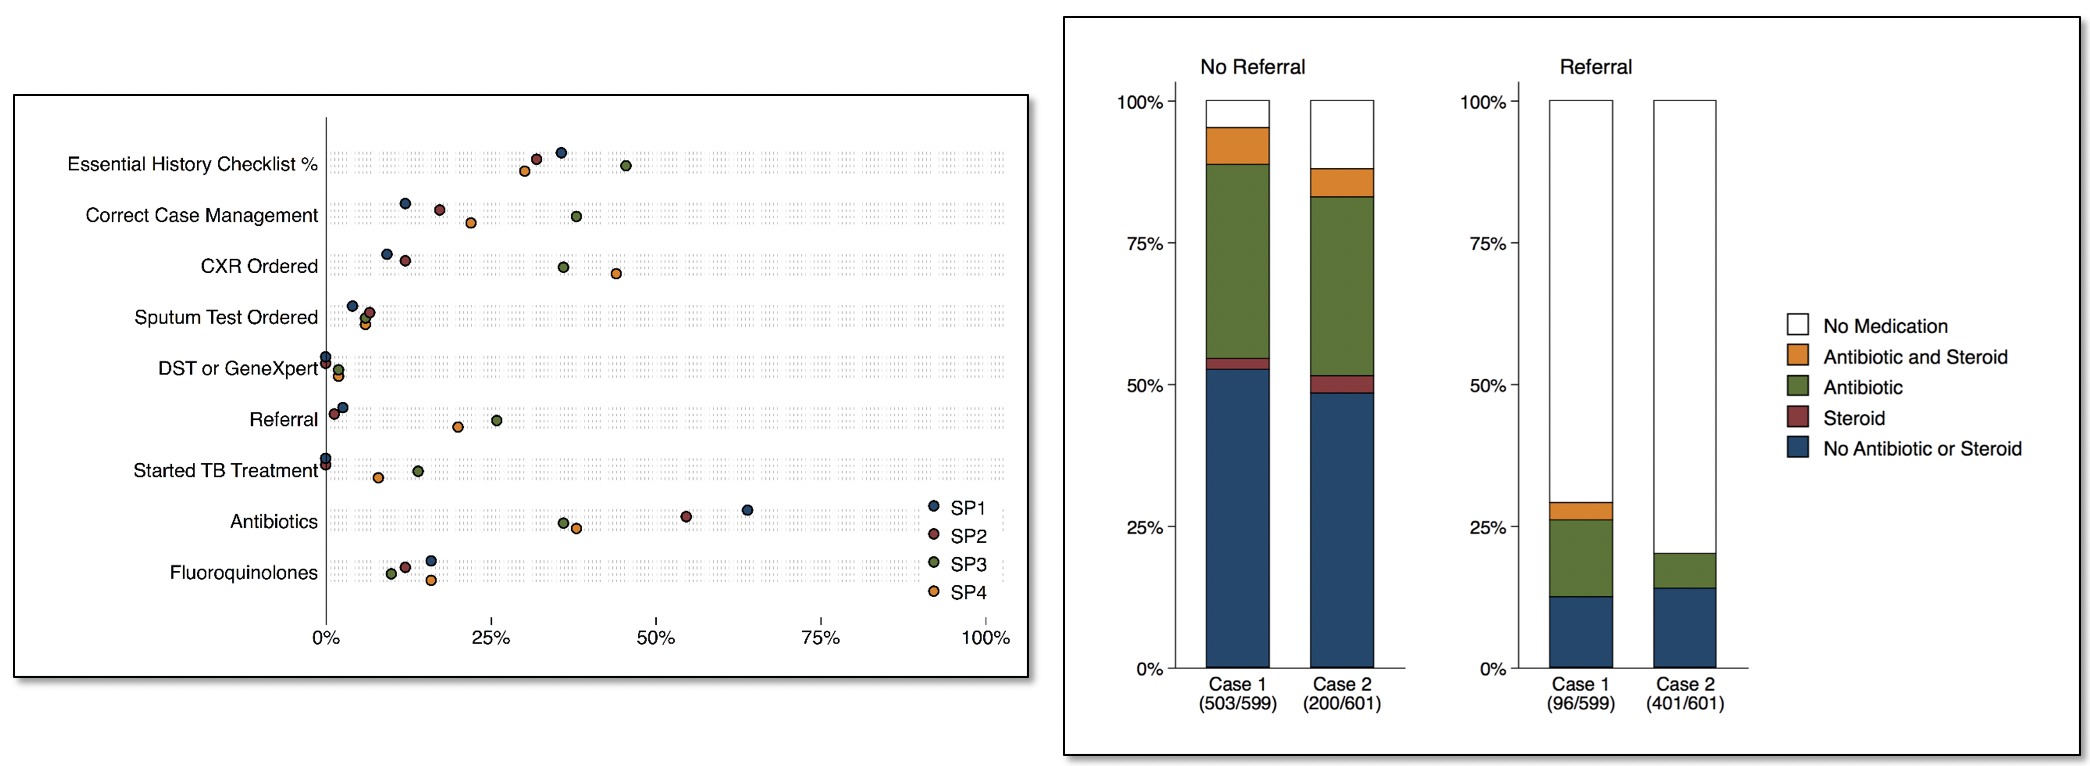
\includegraphics[width=\linewidth]{img/Graph2}
	\end{figure}
	
\end{frame}


\begin{frame}{ \texttt{twoway} graphs can be stacked up}
	\begin{multicols}{2}	
		
		\begin{itemize}[<default overlay specification>]
			\item<1> The axes are abstract, so you do not need to use the same variables or the same units for each graph!
			\item<1> Syntax: 
				\newline \texttt{tw ///}
				\newline \texttt{type var1 var2, opts ///}
				\newline \texttt{type var3 var4, opts ///}
				\newline \texttt{,opts}
			\item<1> Each can have its own  \texttt{if/in} and options.
		\end{itemize}
		
		\begin{figure}
			\centering
			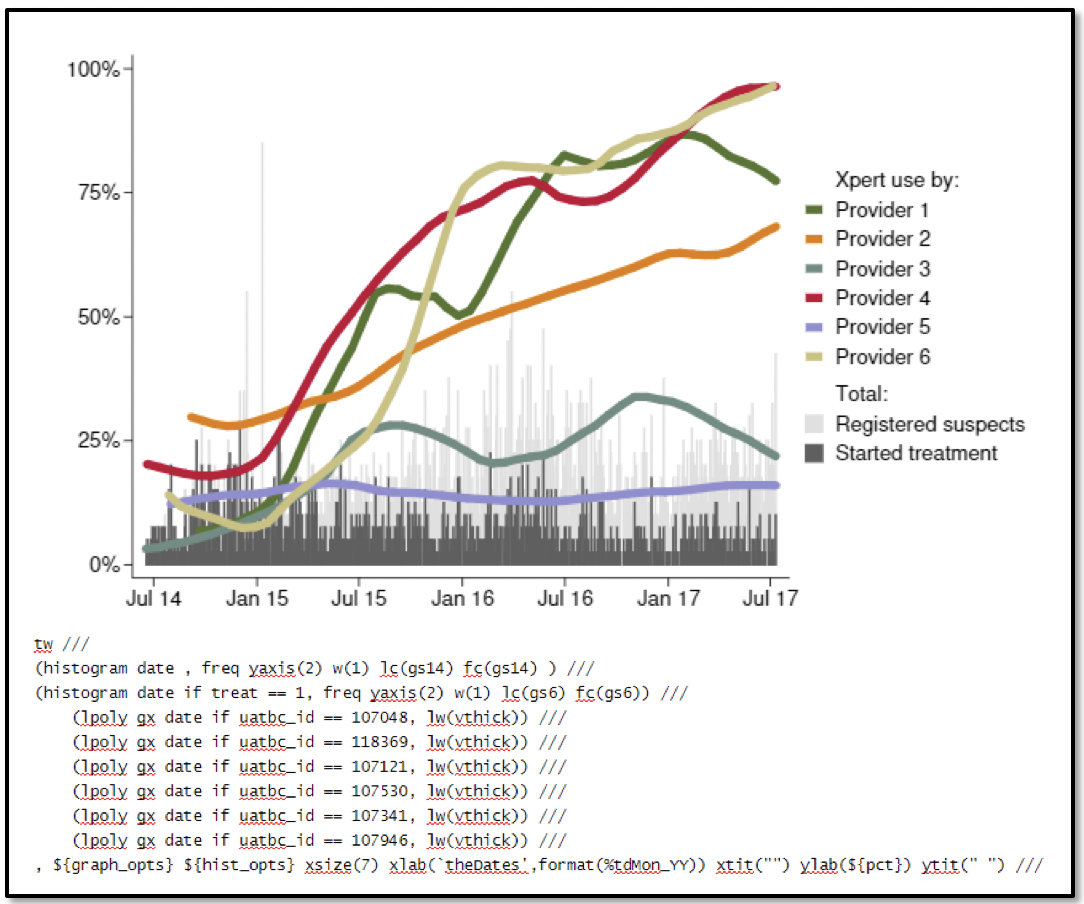
\includegraphics[width=70mm]{img/Graph3}
		\end{figure}
		
	\end{multicols}
\end{frame}


\begin{frame}{Charts show information across dimensions}
	\begin{multicols}{2}	
		
		Not these dimensions!
		
		\begin{figure}
			\centering
			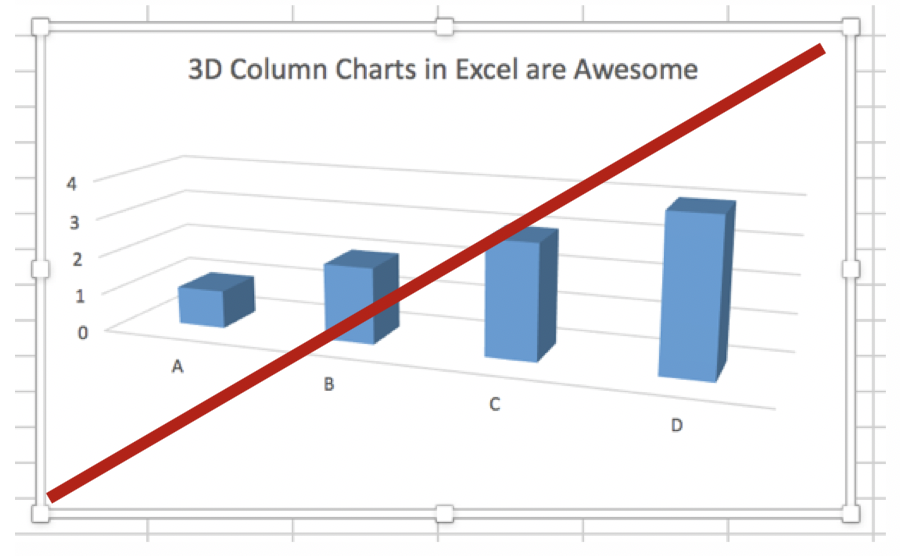
\includegraphics[width=70mm]{img/Dimensions}
		\end{figure}
		
		\begin{figure}
			\centering
			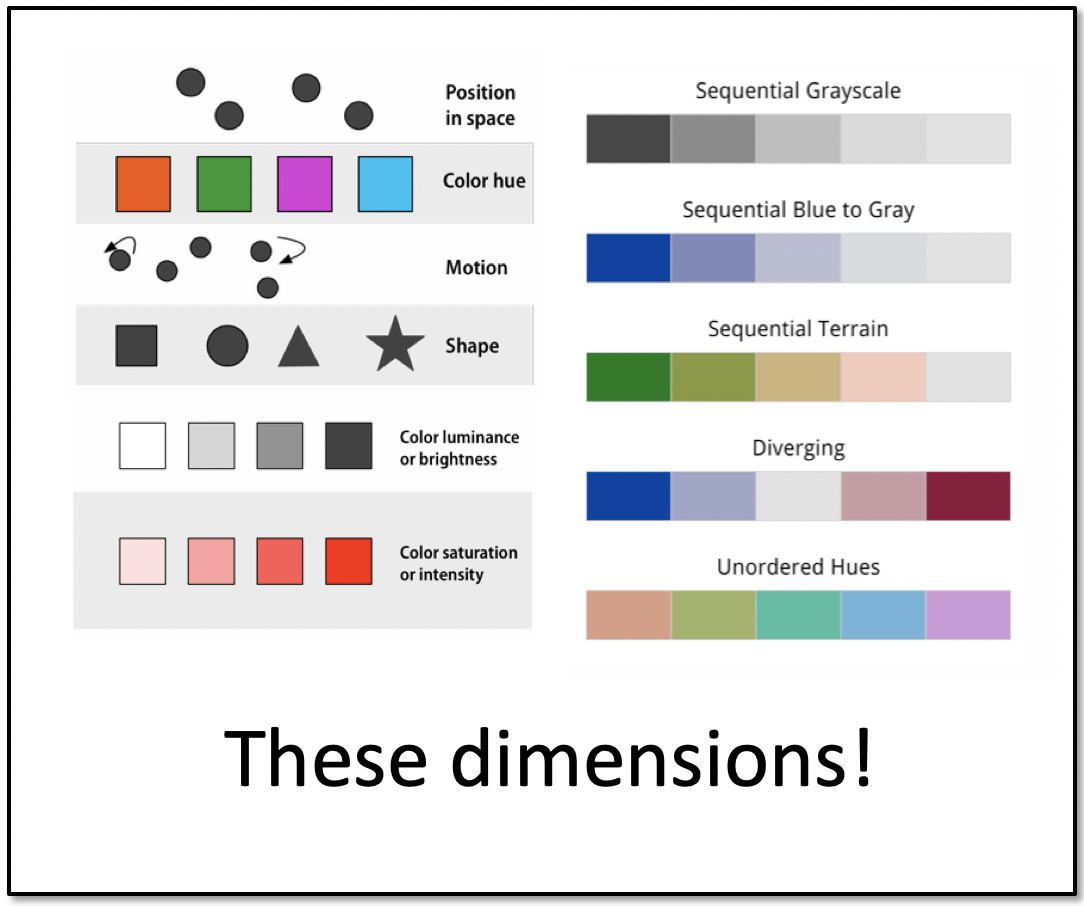
\includegraphics[width=70mm]{img/Dimensions2}
		\end{figure}
		
	\end{multicols}
\end{frame}


\begin{frame}{Design with dimensions in mind}
		
		\begin{itemize}[<default overlay specification>]
			\item<1> A chart with a lot of information can blend together like TV static.
		\end{itemize}
		
		\begin{figure}
			\centering
			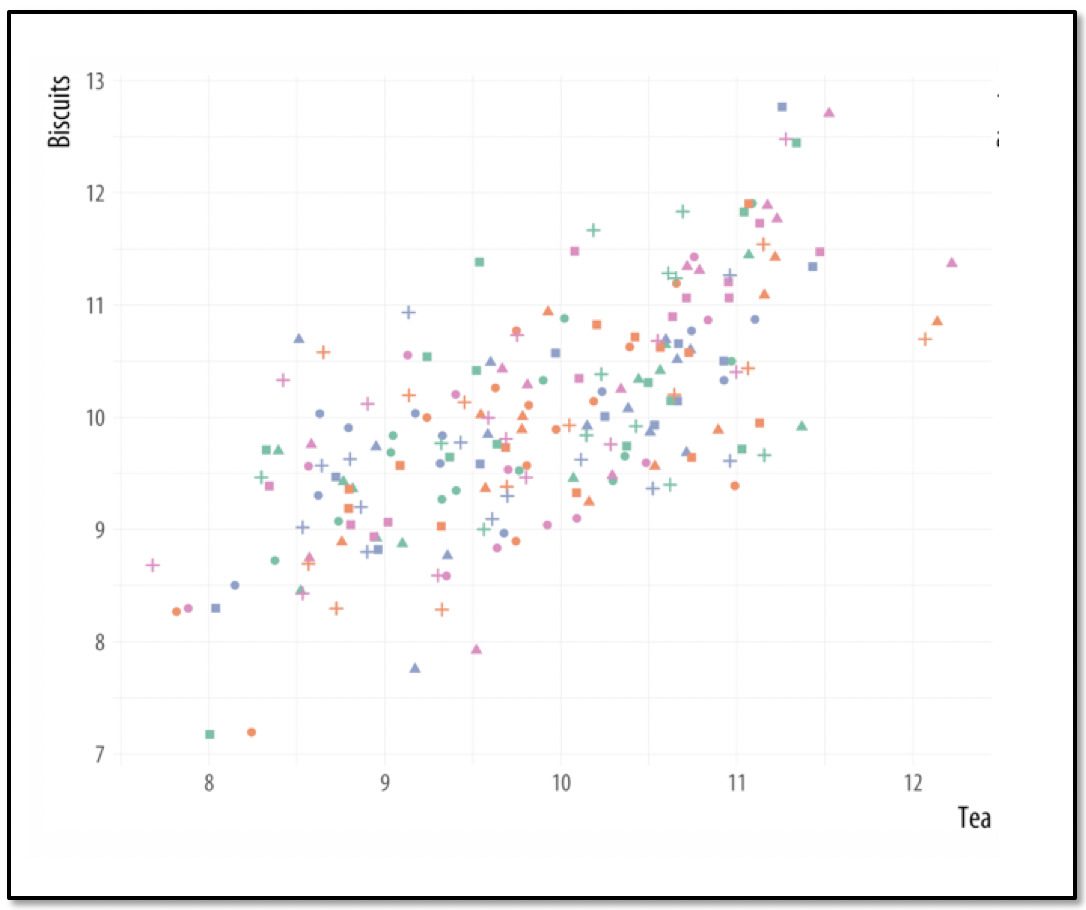
\includegraphics[width=70mm]{img/Dimensions4}
		\end{figure}
		
\end{frame}


\begin{frame}{Use design language to give charts meaning}
	
	\begin{figure}
		\centering
		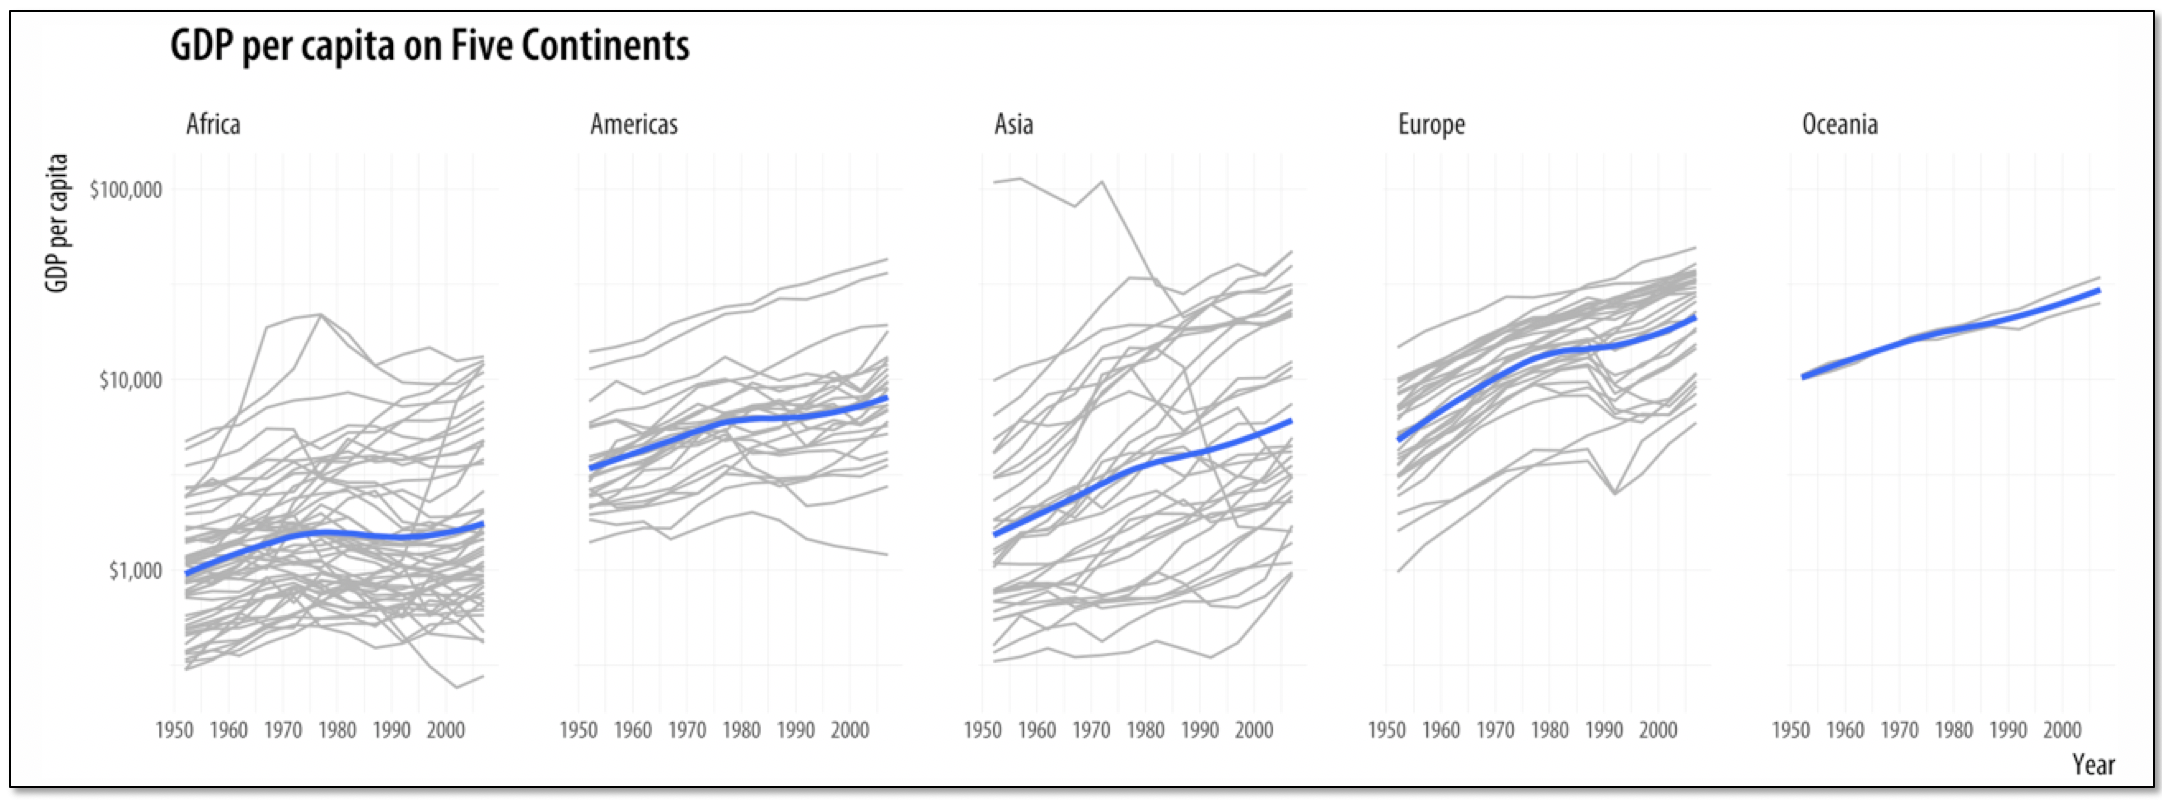
\includegraphics[width=\linewidth]{img/Charts}
	\end{figure}
	
\end{frame}


\begin{frame}{Anatomy of most graphs}
	
	\begin{figure}
		\centering
		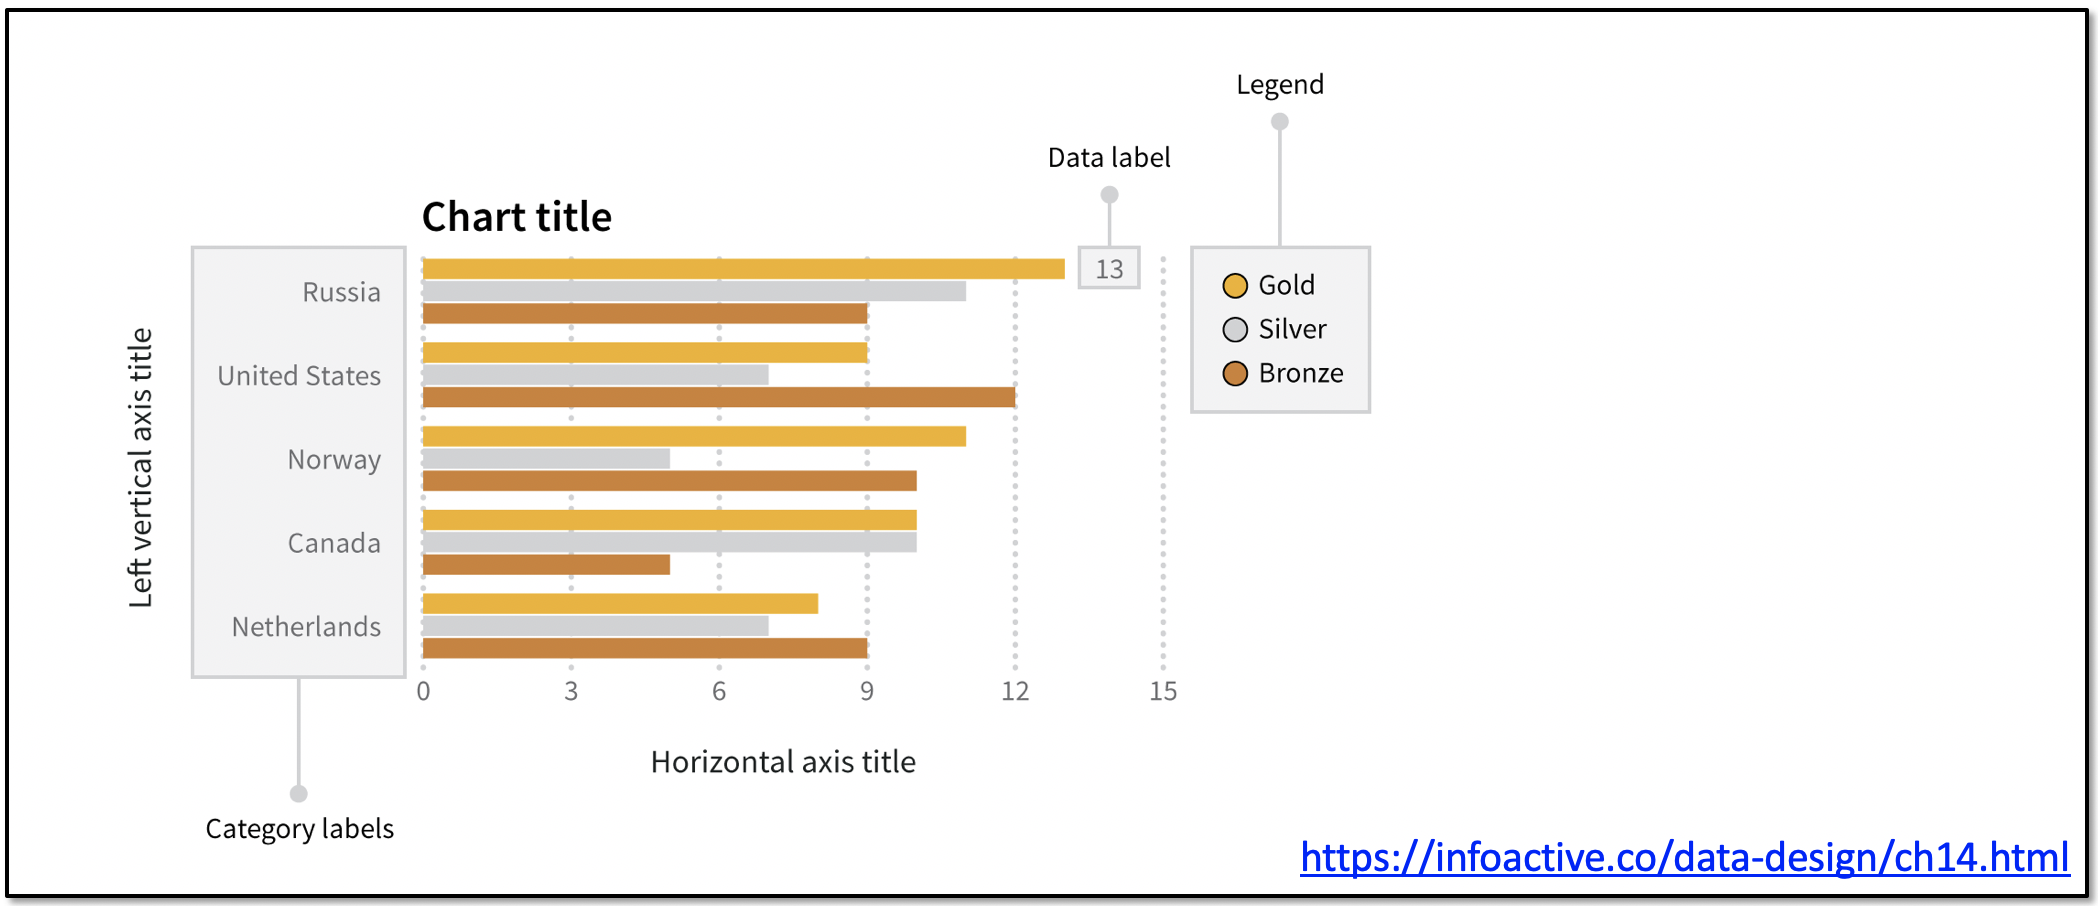
\includegraphics[width=\linewidth]{img/Charts2}
	\end{figure}
	
\end{frame}


\begin{frame}{Components of Stata graphs}
	
	\begin{figure}
		\centering
		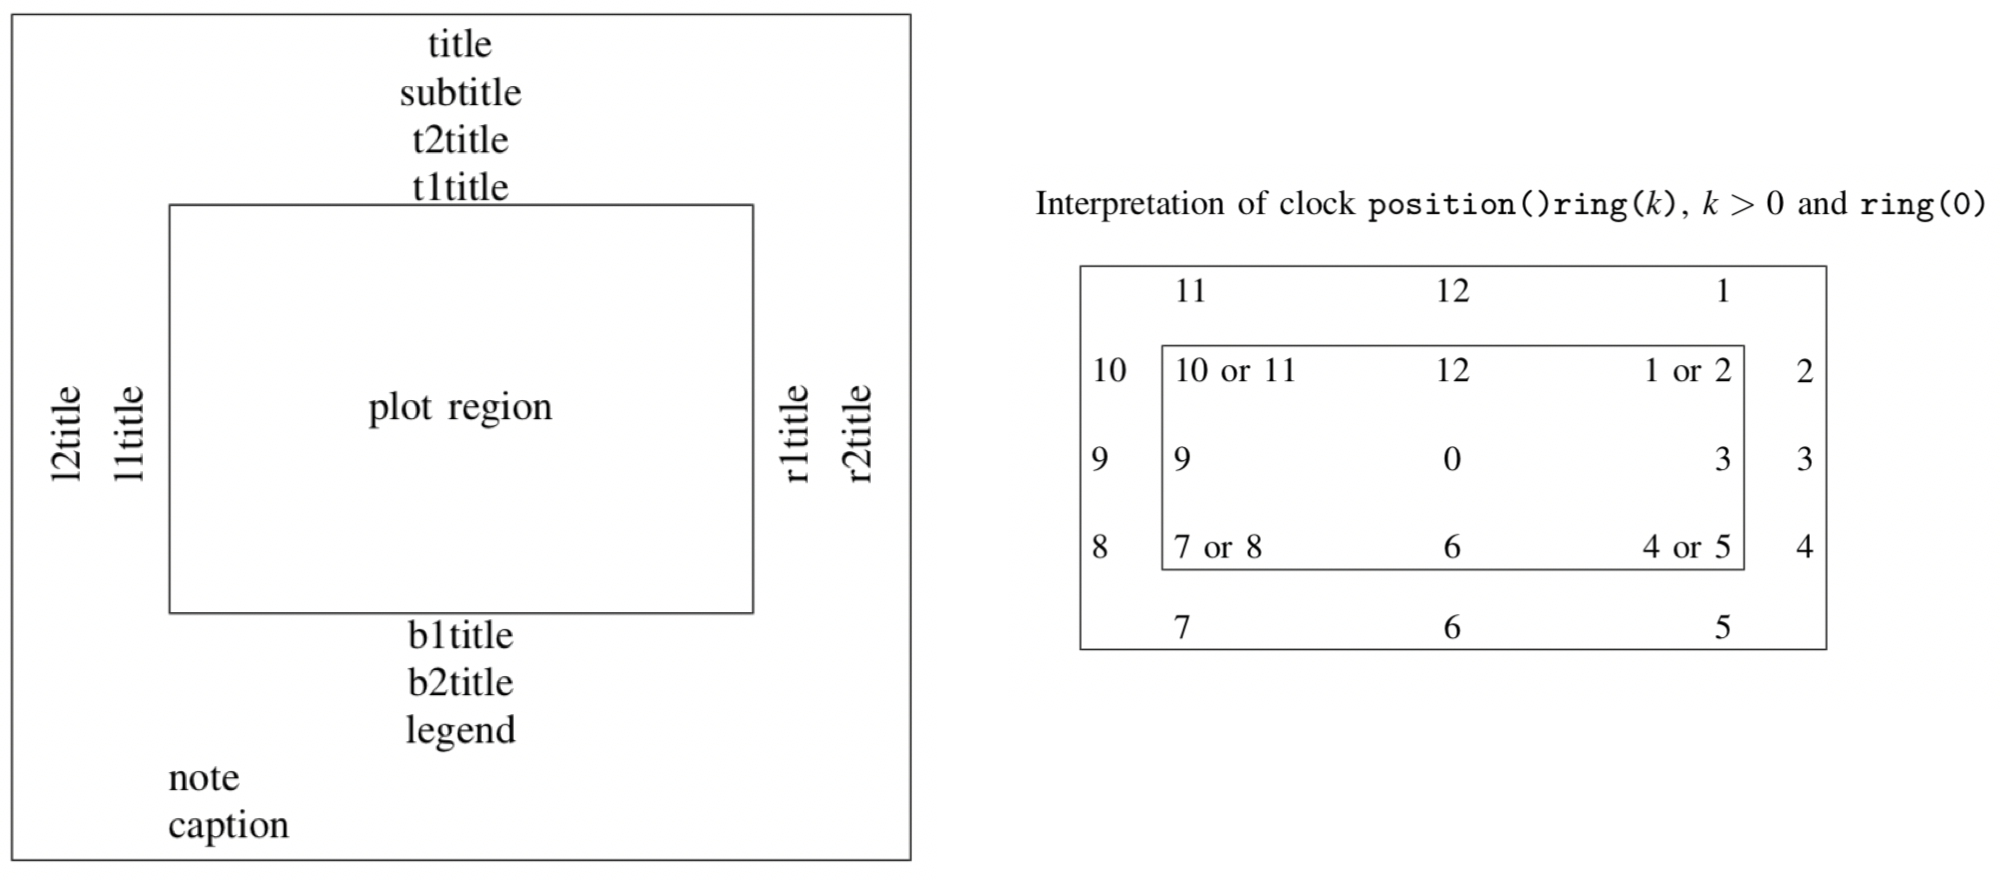
\includegraphics[width=\linewidth]{img/Charts3}
	\end{figure}
	
\end{frame}


\begin{frame}{Best place to start: [h tw]}
	
	\begin{figure}
		\centering
		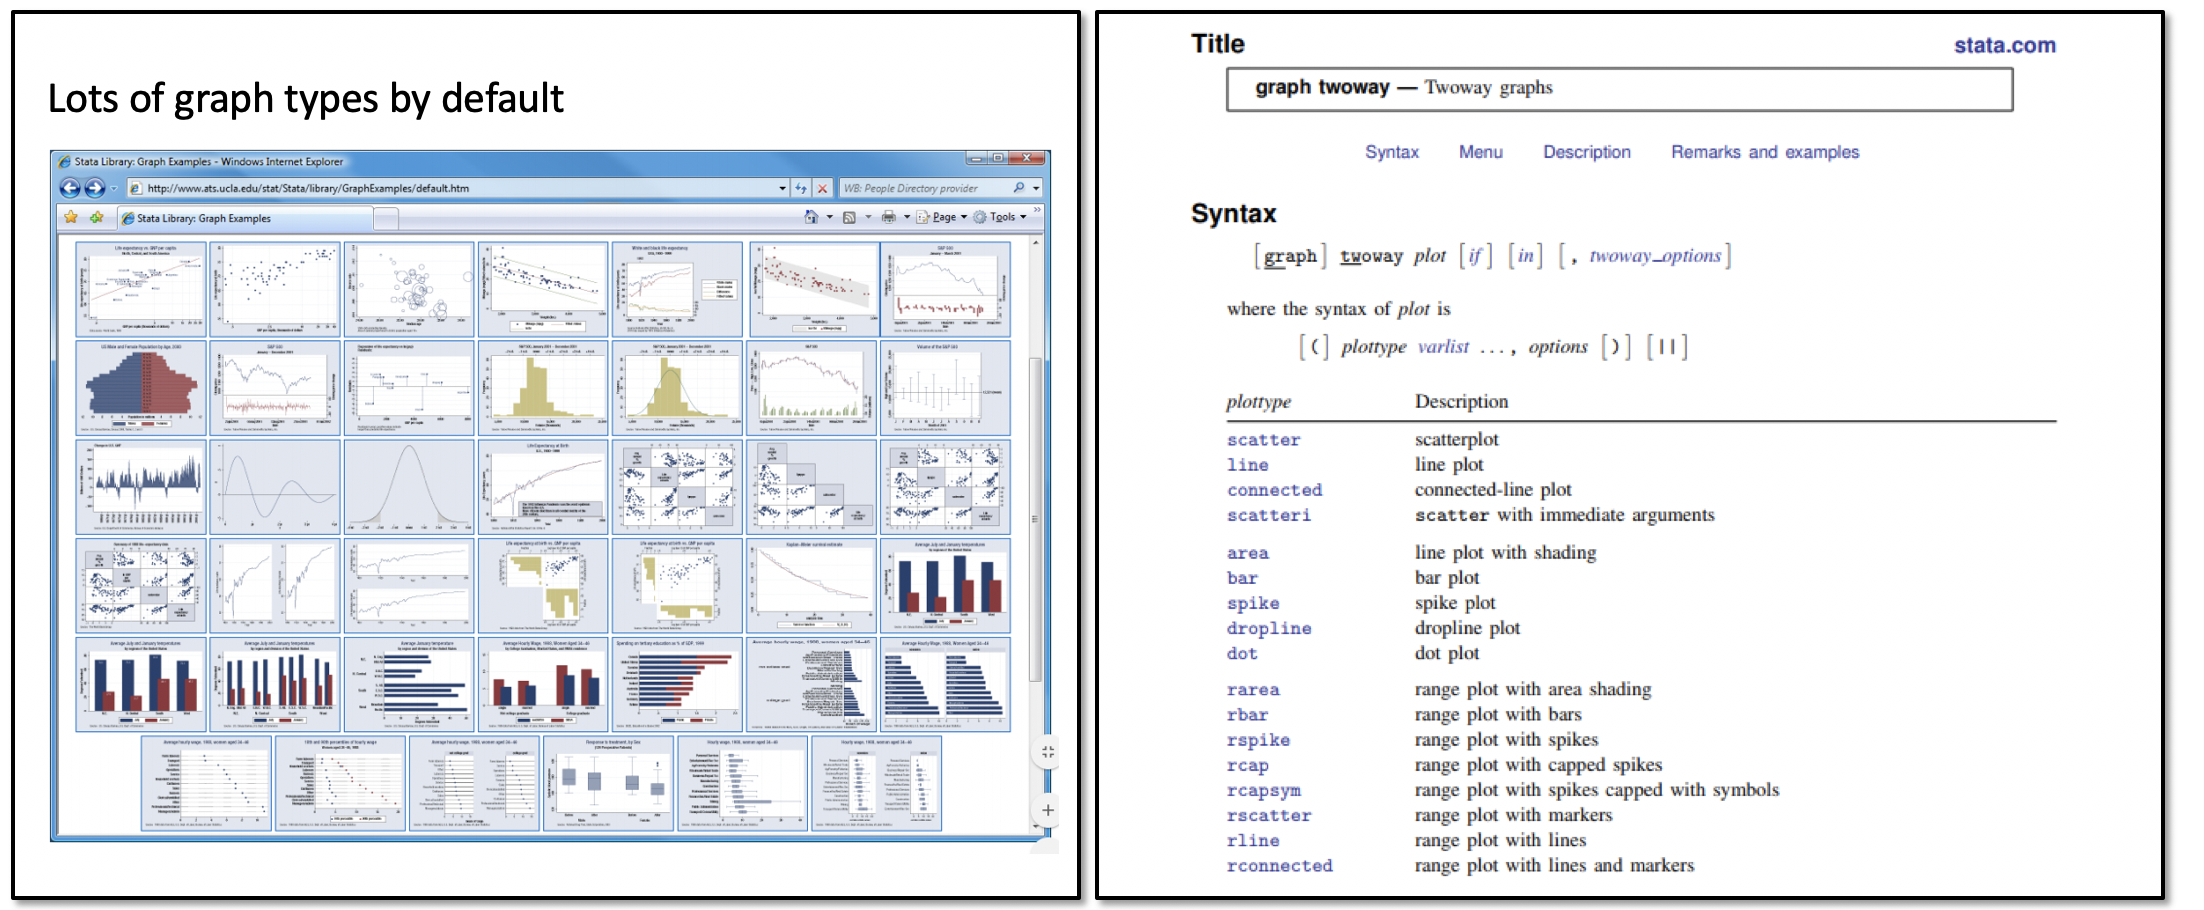
\includegraphics[width=\linewidth]{img/Graphing}
	\end{figure}
	
\end{frame}


\begin{frame}{Best place to start: [h twoway options]}
	\begin{multicols}{2}	
		
		\begin{itemize}[<default overlay specification>]
			\item<1> Major graphing elements:
				\newline - Lines
				\newline - Shapes
				\newline - Points
			\item<1> Major styling elements:
				\newline - Fill color.
				\newline - Outlines
				\newline - Sizes
			\item<1> Major graphing elements
				\newline - Lines
				\newline - Labels
		\end{itemize}
		
		\begin{figure}
			\centering
			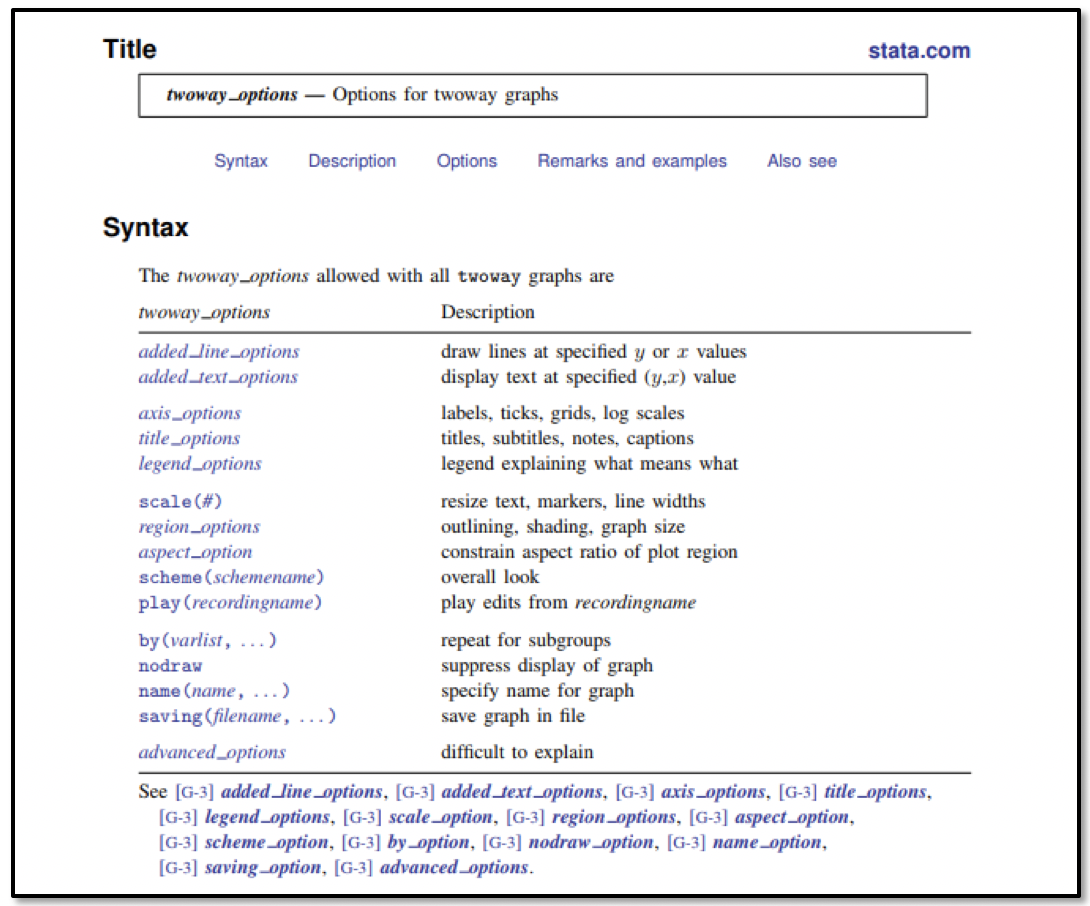
\includegraphics[width=70mm]{img/Graphing2}
		\end{figure}
		
	\end{multicols}
\end{frame}


\begin{frame}{Working with shapes}
	
	\begin{figure}
		\centering
		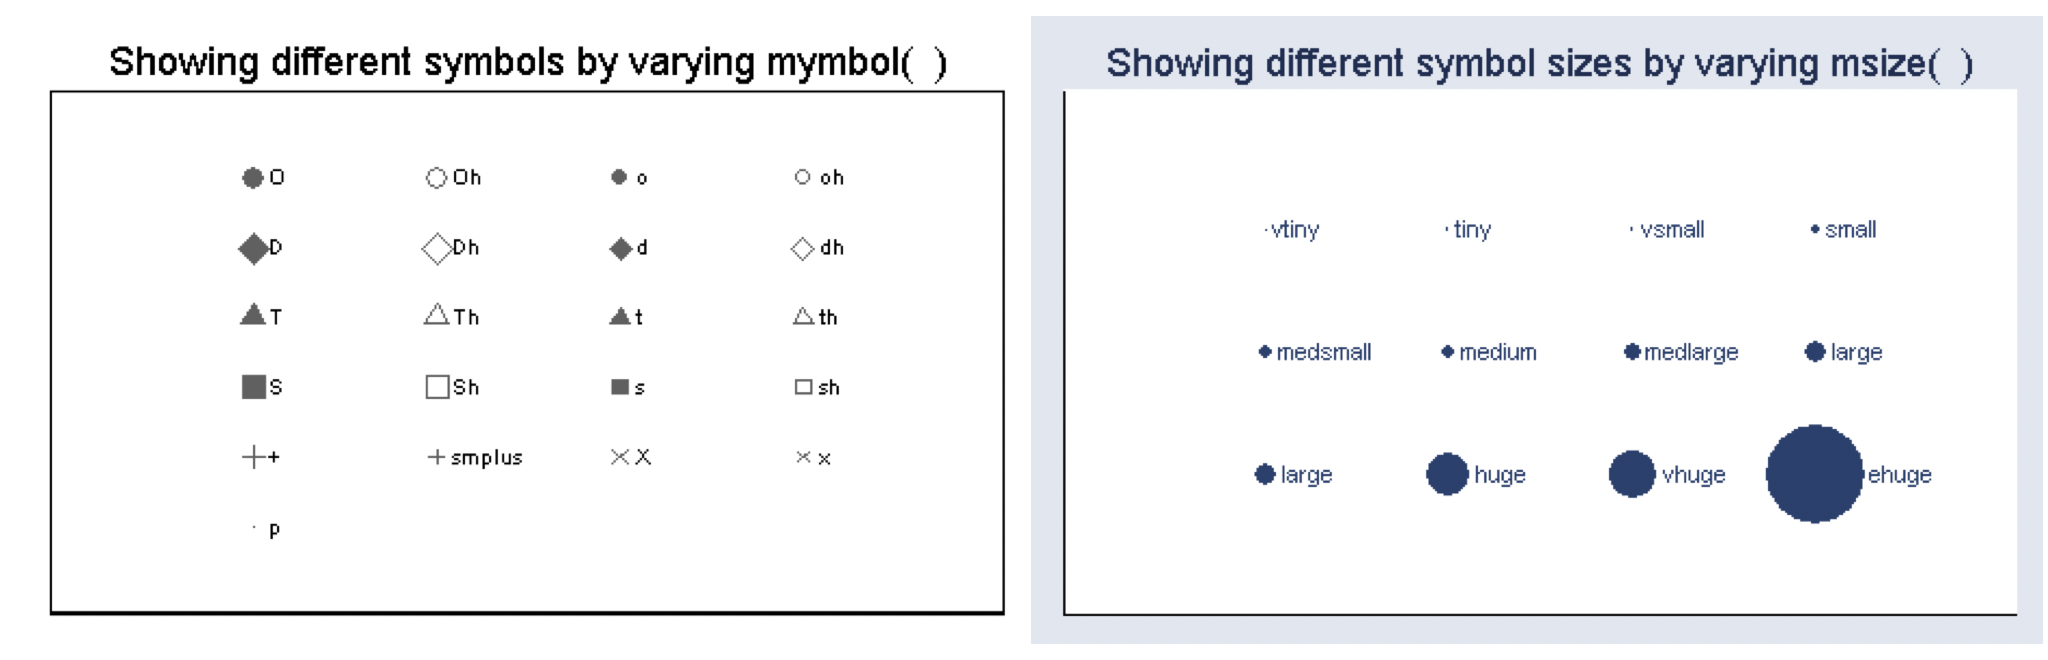
\includegraphics[width=\linewidth]{img/Shapes}
	\end{figure}
	
\end{frame}


\begin{frame}{Working with colors}
	
	\begin{figure}
		\centering
		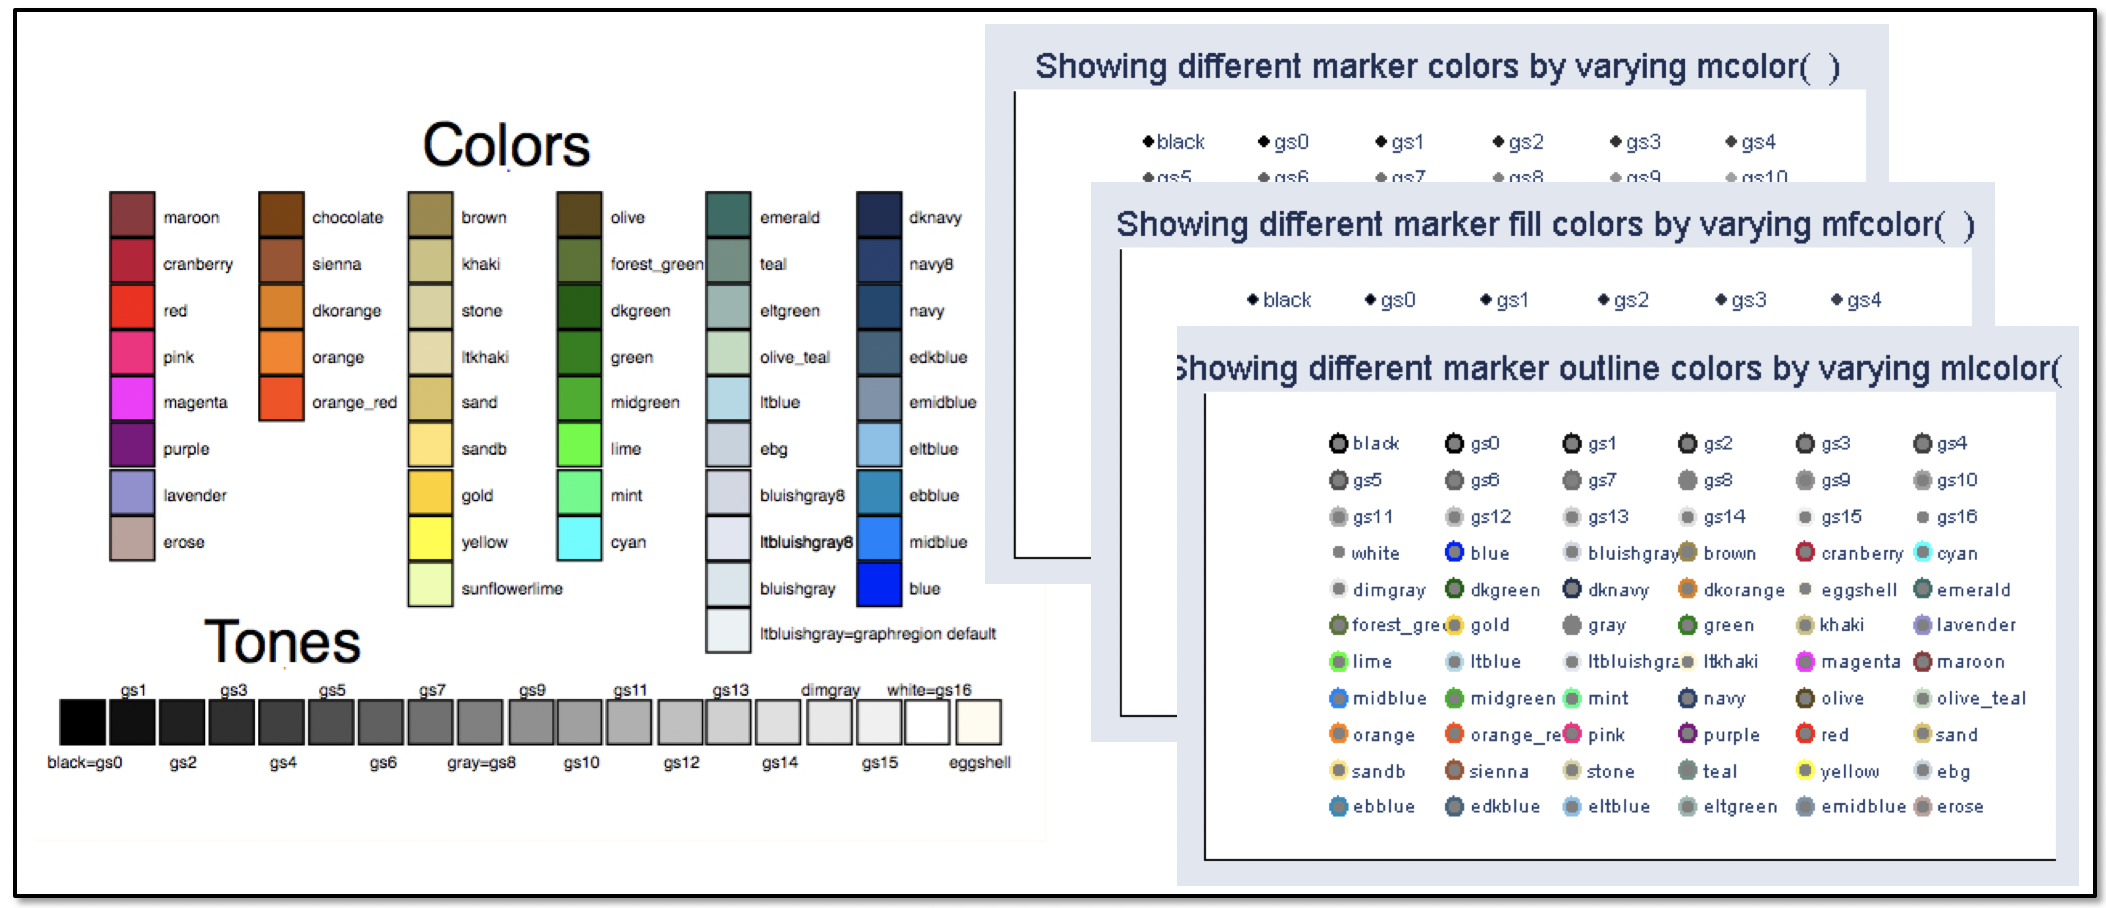
\includegraphics[width=\linewidth]{img/Colors}
	\end{figure}
	
\end{frame}


\begin{frame}{Every graph starts from the basics}
	\begin{multicols}{2}	
		
		\leavevmode 	\newline  \texttt{tw ///}
		 	\newline  \texttt{ (qfitci length weight) ///}
		 	\newline  \texttt{(scatter length weight} 
		 	\newline  \texttt{ if foreign == 0) ///}
		 	\newline  \texttt{(scatter length weight} 
		 	\newline  \texttt{if foreign == 1) }
		
		\begin{figure}
			\centering
			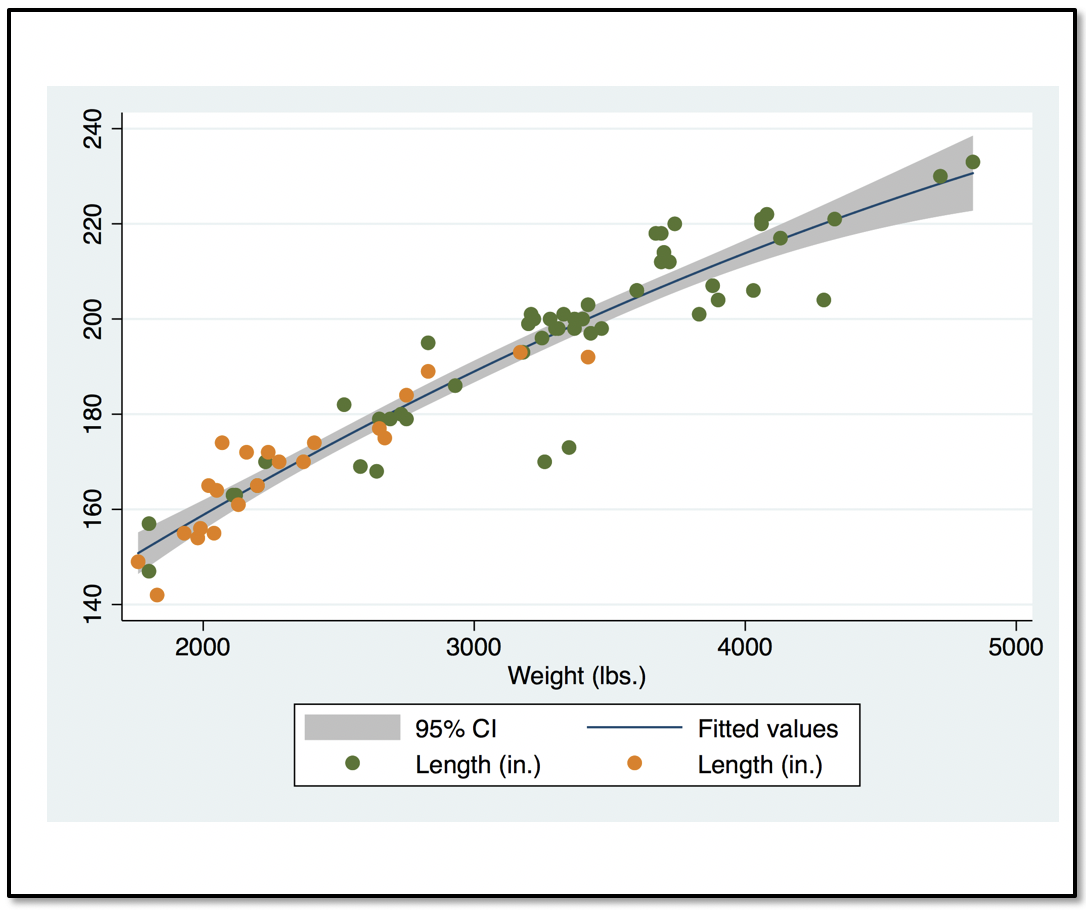
\includegraphics[width=70mm]{img/Basics}
		\end{figure}
		
	\end{multicols}
\end{frame}


\begin{frame}{With styling, we have a pretty graph}
		
	Options … everywhere
		
		\begin{figure}
			\centering
			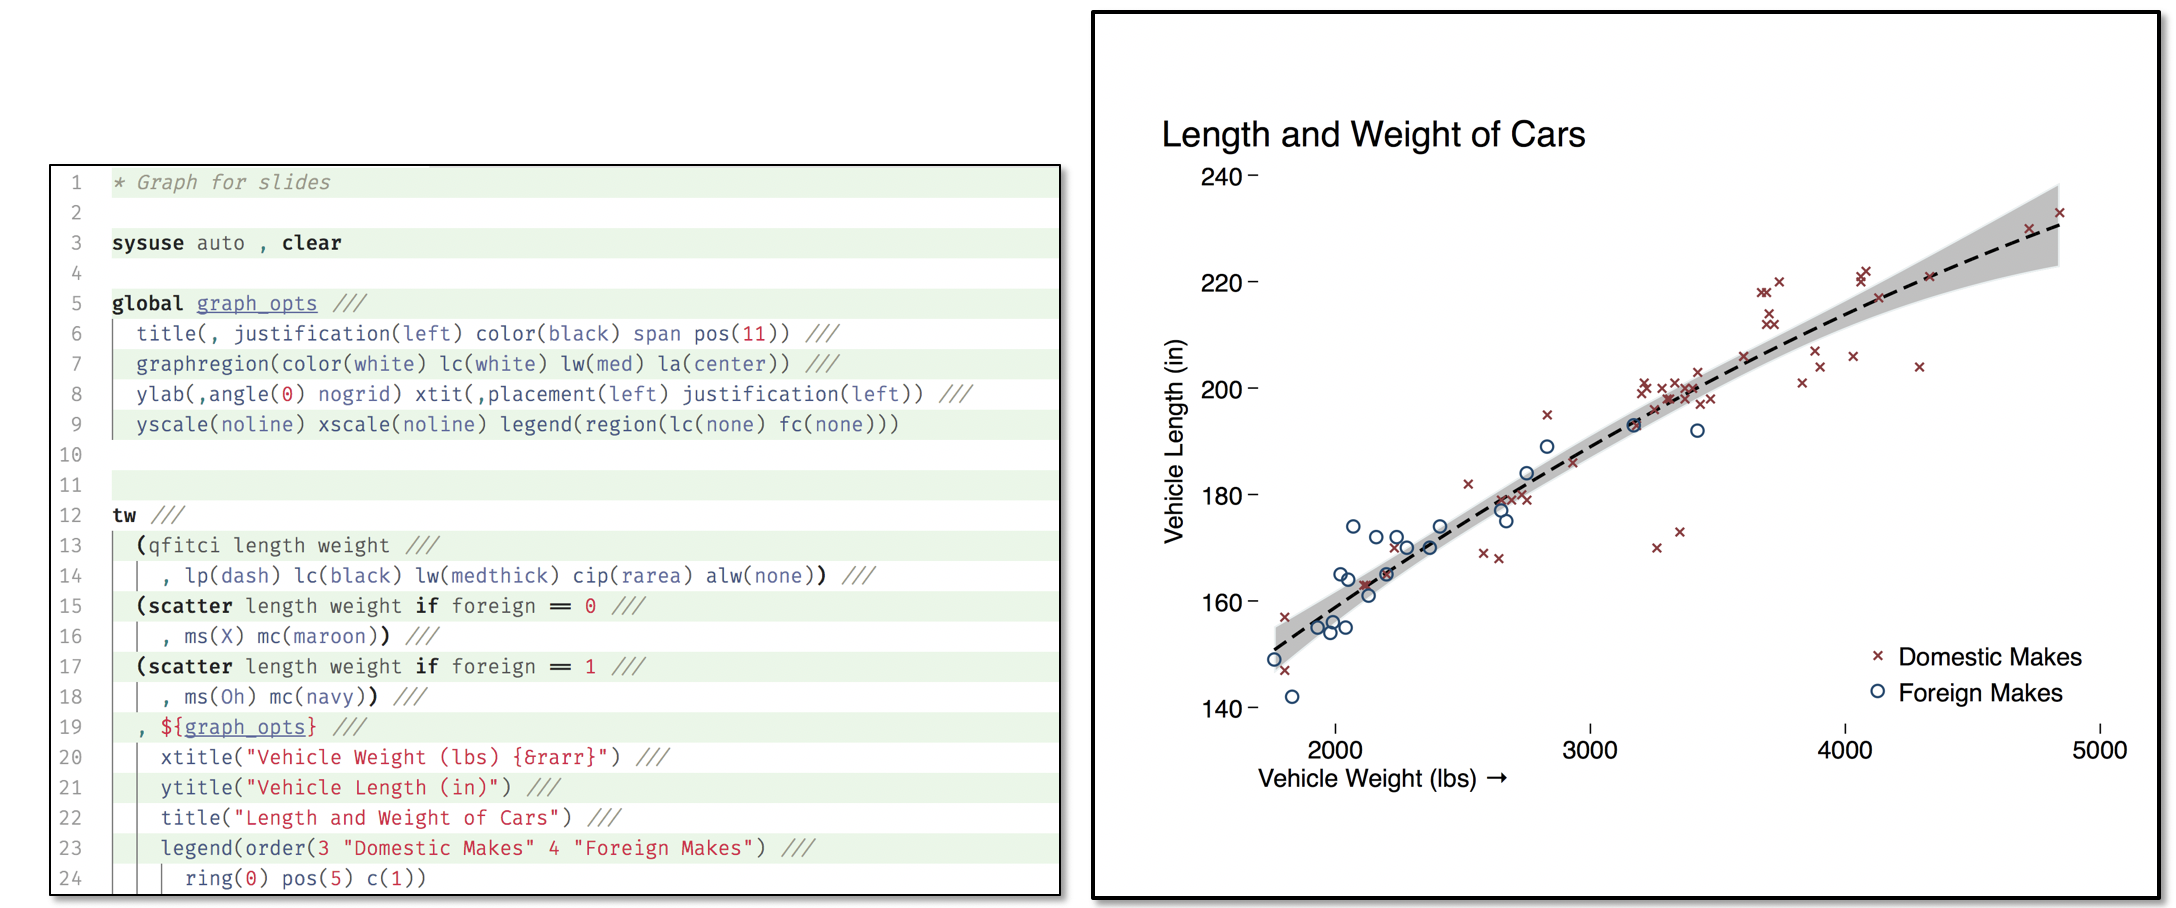
\includegraphics[width=135mm]{img/Styling}
		\end{figure}
		
\end{frame}


\begin{frame}{Graphs can be combined and exported}
	\begin{multicols}{2}	
		
		\leavevmode 	\newline \texttt{graph export ///}

		\leavevmode 	\newline  \texttt{  "filename" /// (.png or .eps)}
		\leavevmode		\newline  \texttt{ (, replace}
 
		\leavevmode		\newline  With .png, specify “width(1000)” for higher resolution
		\newline  .eps files can scale to any size on most modern software (but hard to preview on older systems)
		
		\begin{figure}
			\centering
			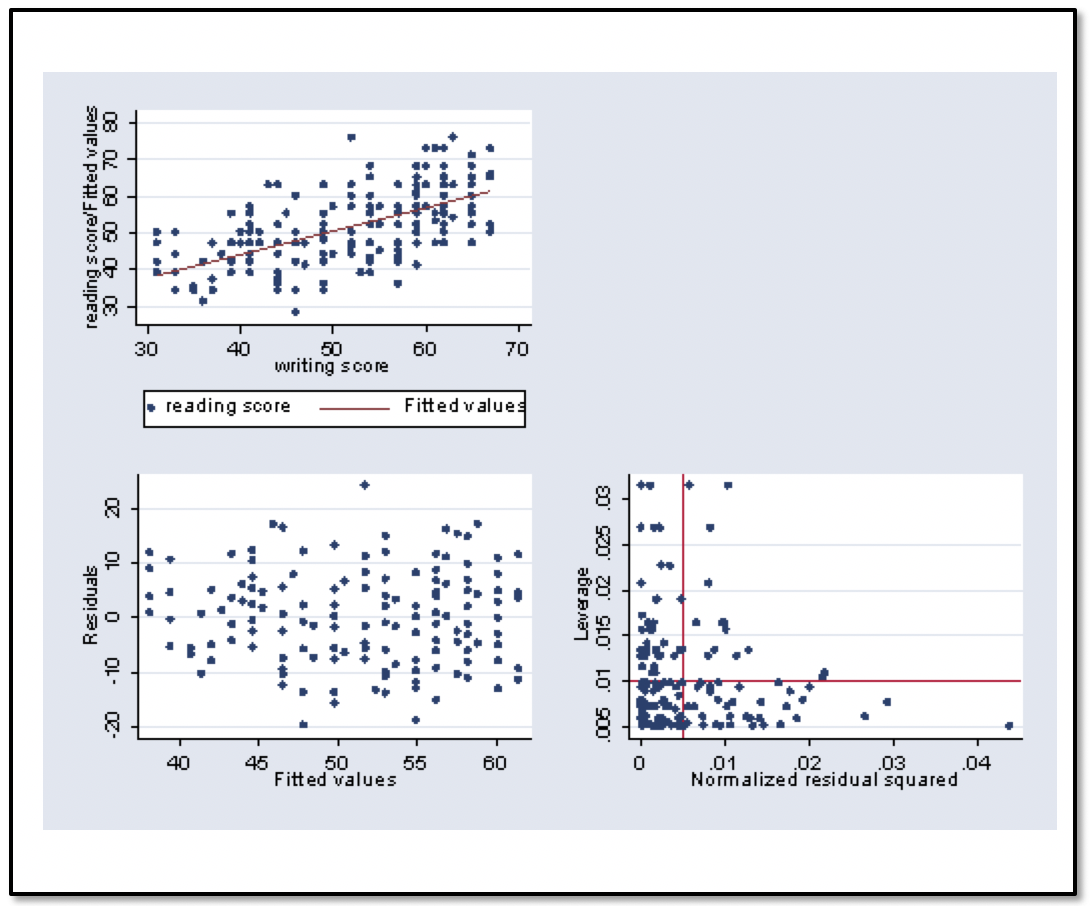
\includegraphics[width=70mm]{img/Styling2}
		\end{figure}
		
	\end{multicols}
\end{frame}


\begin{frame}{DIME Resources (please contribute!)}
	
	\begin{figure}
		\centering
		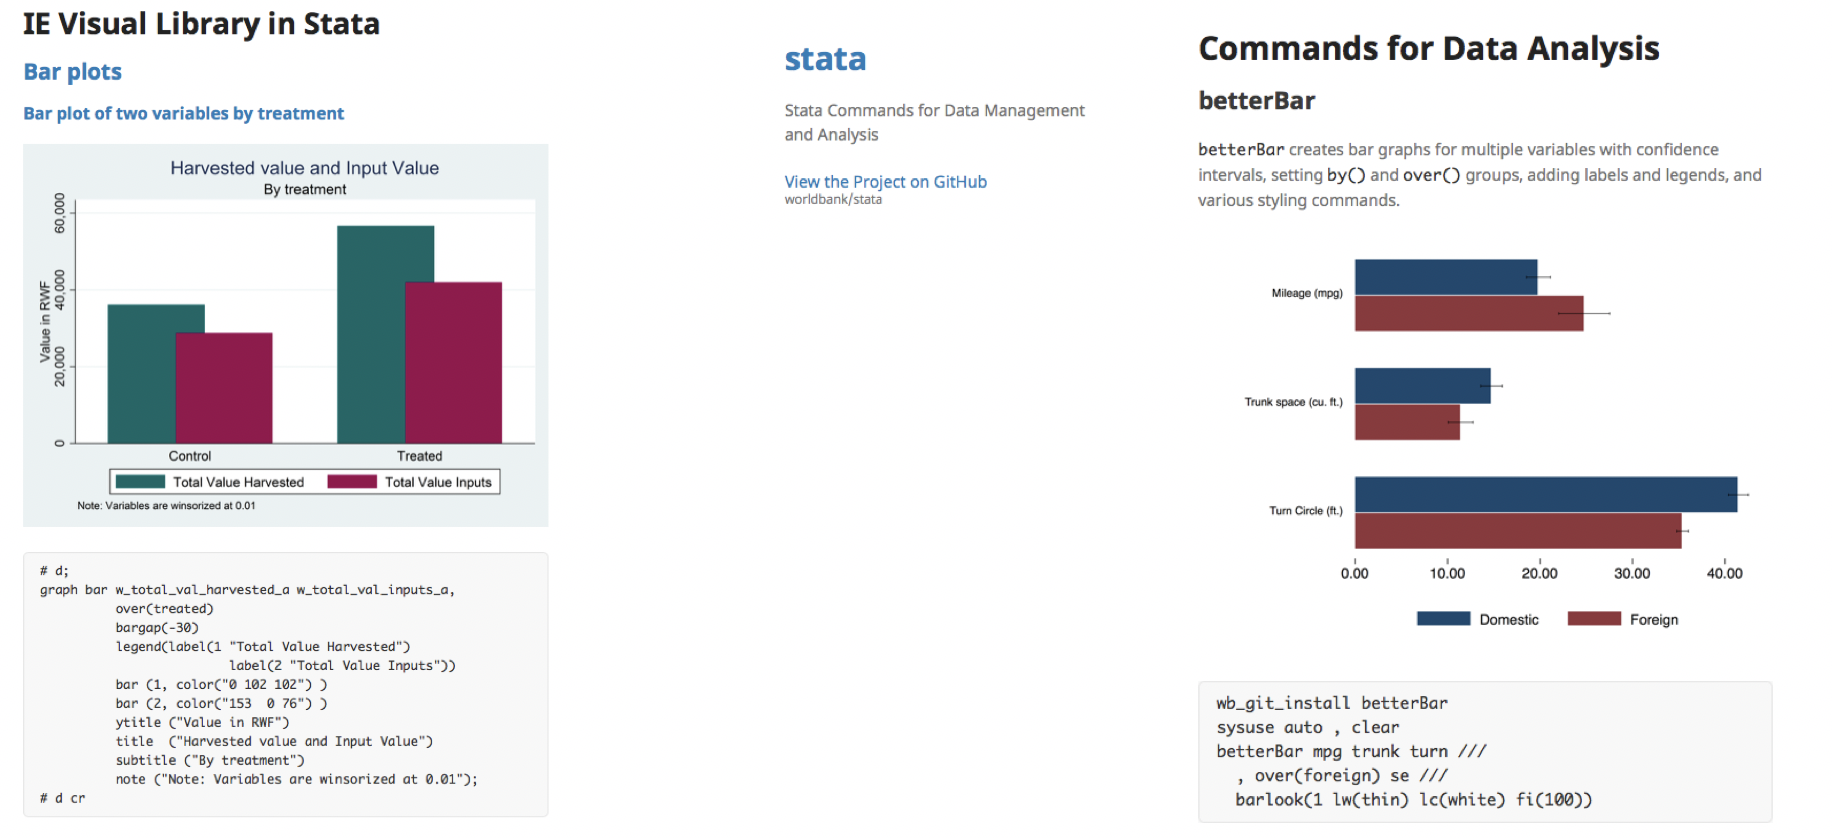
\includegraphics[width=\linewidth]{img/Resources}
	\end{figure}
	
\end{frame}

%%%%%%%%%%%%%%%% Final thougts section %%%%%%%%%%%%%%%%%%
\begin{frame}{Conclusion}

Thank You!

\vspace{20mm}
For more information or further questions please contact:
\newline Benjamin Daniels (\url{bdaniels@worldbank.org}) 

\end{frame}

%%%%%%%%%%%%%%%%%%%%%%%%%%%%%%%%%%%%%%%%%%% The End
\sectionpic{The End}{img/section_slide}






\end{document} 